%%%%%%%%%%%%%%%%%%%%%%%%%%%%%%%%%%%%%%%%%%%%%%%%%%%%%%%%%%
%   Autoren:
%   Prof. Dr. Bernhard Drabant
%   Prof. Dr. Dennis Pfisterer
%   Prof. Dr. Julian Reichwald
%%%%%%%%%%%%%%%%%%%%%%%%%%%%%%%%%%%%%%%%%%%%%%%%%%%%%%%%%%

%%%%%%%%%%%%%%%%%%%%%%%%%%%%%%%%%%%%%%%%%%%%%%%%%%%%%%%%%%
%	ANLEITUNG: 
%   1. Ersetzen Sie firmenlogo.jpg im Verzeichnis img
%   2. Passen Sie alle Stellen im Dokument an, die mit 
%      @stud 
%      markiert sind
%%%%%%%%%%%%%%%%%%%%%%%%%%%%%%%%%%%%%%%%%%%%%%%%%%%%%%%%%%

%%%%%%%%%%%%%%%%%%%%%%%%%%%%%%%%%%%%%%%%%%%%%%%%%%%%%%%%%%
%	ACHTUNG: 
%   Für das Erstellen des Literaturverzeichnisses wird das 
%   modernere Paket biblatex in Kombination mit biber 
%   verwendet - nicht mehr das ältere Paket BibTex!
%
%   Bitte stellen Sie Ihre TeX-Umgebung entsprechend ein (z.B. TeXStudio): 
%   Einstellungen --> Erzeugen --> Standard Bibliographieprogramm: biber
%%%%%%%%%%%%%%%%%%%%%%%%%%%%%%%%%%%%%%%%%%%%%%%%%%%%%%%%%%

\documentclass[fontsize=12pt,BCOR=5mm,DIV=12,parskip=half,listof=totoc,
               paper=a4,toc=bibliography,pointlessnumbers]{scrreprt}
               
               %toc=listof,listof=entryprefix,
               
\makeindex

%% Elementare Pakete, Konfigurationen und Definitionen werden geladen (gegebenenfalls anpassen)
% !TEX root =  master.tex

%%%%%%%%%%%%%%%%%%%%%%%%%%%%%%%%%%%%%%%%%%%%%%%%%%%%%%%%%%%%%%%%%%
%	ANLEITUNG: 
% Passen Sie gegebenenfalls alle Stellen im Dokument an, die mit 
% @stud 
% markiert sind.
%%%%%%%%%%%%%%%%%%%%%%%%%%%%%%%%%%%%%%%%%%%%%%%%%%%%%%%%%%%%%%%%%%

%%
%% @stud
%%
%% LANGUAGE SETTINGS
\usepackage[ngerman]{babel} 	        % german language
\usepackage[german=quotes]{csquotes} 	% correct quoting using \enquote{}
%\usepackage[english]{babel}          % english language
%\usepackage{csquotes} 	              % correct quoting using \enquote{}
\usepackage{eurosym}
\usepackage{makeidx}                  % allows index generation
\usepackage{listings}	                %Format Listings properly
\usepackage{lipsum}                   % Blindtext
\usepackage{graphicx}       
\usepackage{tabularx}                          % use various graphics formats
\usepackage[german]{varioref}
\usepackage{caption}	                % better Captions
\usepackage{booktabs}                 % nicer Tabs
\usepackage[hidelinks=true]{hyperref} % keine roten Markierungen bei Links
\usepackage{fnpct}                    % Correct superscripts 
\usepackage{calc}                     % Used for extra space below footsepline, in particular
\usepackage{array}
\usepackage{acronym}
\usepackage{algorithm}
\usepackage{algpseudocode}
\usepackage{setspace}
\usepackage{tocloft}
\usepackage{makecell}
\usepackage{hhline}

\usepackage{longtable}
\usepackage{svg}
\usepackage{amssymb}

%Benedikt
\usepackage{xltabular}

% Davids Abschnitt
\usepackage{geometry}
\usepackage{pdflscape}
\usepackage{wrapfig}

%% Schriftarten- und Zeichenpakete
\usepackage[T1]{fontenc}
\usepackage[utf8]{inputenc}

%%
%% @stud
%%
%%	FONT SELECTION: Schriftarten und Schriftfamilie
%%%%%%%%%%%%%
%% SCHRIFTART
%%%%%%%%%%%%%
% 0) without decomment: normal font families 
% ...
% 1) Latin Modern 
\usepackage{lmodern}        
% 2) Times 
%\usepackage{mathptmx}         
% 3) Helvetica
%\usepackage[scaled=.92]{helvet} 
%%%%%%%%%%%%%%%%%%
%%	SCHRIFTFAMILIE
%%%%%%%%%%%%%%%%%%
% ohne Serifen
\renewcommand*{\familydefault}{\sfdefault}
\addtokomafont{disposition}{\sffamily}
%
% mit Serifen
%\renewcommand*{\familydefault}{\rmdefault}
%\addtokomafont{disposition}{\rmfamily}
%
% Typewriter
%\renewcommand*{\familydefault}{\ttdefault}
%\addtokomafont{disposition}{\ttfamily}

%%
%% @stud
%%
%% Uncomment the following lines to support hard URL breaks in bibliography 
%\apptocmd{\UrlBreaks}{\do\f\do\m}{}{}
%\setcounter{biburllcpenalty}{9000}% Kleinbuchstaben
%\setcounter{biburlucpenalty}{9000}% Großbuchstaben

%%
%% @stud
%%
%% FOOTNOTES: Count footnotes over chapters
%% \counterwithout{footnote}{chapter}

%	ACRONYMS
\makeatletter
\@ifpackagelater{acronym}{2015/03/20}
{\renewcommand*{\aclabelfont}[1]{\textbf{{\acsfont{#1}}}}}{}
\makeatother

%	LISTINGS
% @stud: ggf. Namen/Text anpassen (englisch)
\renewcommand{\lstlistingname}{Quelltext} 
\renewcommand{\lstlistlistingname}{Quelltextverzeichnis}
\lstset{numbers=left,
	numberstyle=\tiny,
	captionpos=b,
	basicstyle=\ttfamily\small}

%	ALGORITHMS
% @stud: ggf. Namen/Text anpassen (englisch)
\renewcommand{\listalgorithmname}{Algorithmenverzeichnis}
\floatname{algorithm}{Algorithmus}

%	PAGE HEADER / FOOTER
%	Warning: There are some redefinitions throughout the master.tex-file!  DON'T CHANGE THESE REDEFINITIONS!
\RequirePackage[automark]{scrlayer-scrpage}
%alternatively with separation lines: \RequirePackage[automark,headsepline,footsepline]{scrlayer-scrpage}

\renewcommand{\chaptermarkformat}{}
\RedeclareSectionCommand[beforeskip=0pt]{chapter}
\clearpairofpagestyles

%\ifoot[\rule{0pt}{\ht\strutbox+\dp\strutbox}DHBW Mannheim]{\rule{0pt}{\ht\strutbox+\dp\strutbox}DHBW Mannheim}
\ofoot[\rule{0pt}{\ht\strutbox+\dp\strutbox}\pagemark]{\rule{0pt}{\ht\strutbox+\dp\strutbox}\pagemark}
\ohead{\headmark}

\newcommand{\TitelDerArbeit}[1]{\def\DerTitelDerArbeit{#1}\hypersetup{pdftitle={#1}}}
\newcommand{\AutorDerArbeit}[1]{\def\DerAutorDerArbeit{#1}\hypersetup{pdfauthor={#1}}}
\newcommand{\Firma}[1]{\def\DerNameDerFirma{#1}}
\newcommand{\Kurs}[1]{\def\DieKursbezeichnung{#1}}
\newcommand{\Abteilung}[1]{\def\DerNameDerAbteilung{#1}}
\newcommand{\Studiengangsleiter}[1]{\def\DerStudiengangsleiter{#1}}
\newcommand{\WissBetreuer}[1]{\def\DerWissBetreuer{#1}}
\newcommand{\FirmenBetreuer}[1]{\def\DerFirmenBetreuer{#1}}
\newcommand{\Bearbeitungszeitraum}[1]{\def\DerBearbeitungszeitraum{#1}}
\newcommand{\Abgabedatum}[1]{\def\DasAbgabedatum{#1}}
\newcommand{\Matrikelnummer}[1]{\def\DieMatrikelnummer{#1}}
\newcommand{\Studienrichtung}[1]{\def\DieStudienrichtung{#1}}
\newcommand{\ArtDerArbeit}[1]{\def\DieArtDerArbeit{#1}}
\newcommand{\Literaturverzeichnis}{Literaturverzeichnis}

\newcommand{\settingBibFootnoteCite}{
	\setlength{\bibparsep}{\parskip}		  % Add some space between biblatex entries in the bibliography
	\addbibresource{bibliography.bib}	    % Add file bibliography.bib as biblatex resource
	\DefineBibliographyStrings{ngerman}{andothers = {{et\,al\adddot}},}
}

\newcommand{\setTitlepage}{
	% !TEX root =  master.tex
% @stud: ggf. Namen/Text anpassen (englisch)
\begin{titlepage}
\begin{minipage}{\textwidth}
		\vspace{-2cm}
		\noindent \hfill 
\includegraphics{\imagedir/logo.jpg}
\end{minipage}
\vspace{1em}
%\sffamily
\begin{center}
	{\textsf{\large Duale Hochschule Baden-W\"urttemberg Mannheim}}\\[4em]
	{\textsf{\textbf{\large{\DieArtDerArbeit}arbeit}}}\\[6mm]
	{\textsf{\textbf{\Large{}\DerTitelDerArbeit}}} \\[1.5cm]
	{\textsf{\textbf{\large{}Studiengang Wirtschaftsinformatik}}\\[6mm]
	\textsf{\textbf{Studienrichtung \DieStudienrichtung}}}\vspace{15em}
	
	\begin{minipage}{\textwidth}
		\begin{tabbing}
		Wissenschaftliche(r) Betreuer(in): \hspace{0.85cm}\=\kill
		Verfasser: \> \DerAutorDerArbeit \\[1.5mm]
		Matrikelnummer: \> \DieMatrikelnummer \\[1.5mm]
%		Firma: \> \DerNameDerFirma  \\[1.5mm]
%		Abteilung: \> \DerNameDerAbteilung \\[1.5mm]
		Kurs: \> \DieKursbezeichnung \\[1.5mm]
		Studiengangsleiter: \> \DerStudiengangsleiter \\[1.5mm]
		Dozent: \> \DerWissBetreuer \\[1.5mm]
%		Firmenbetreuer(in): \> \DerFirmenBetreuer \\[1.5mm]
		Bearbeitungszeitraum: \> \DerBearbeitungszeitraum\\[1.5mm]
%		alternativ:\\[1.5mm]
%		Eingereicht: \> \DasAbgabedatum	
		\end{tabbing}
	\end{minipage}
\end{center}
\end{titlepage}
	\pagenumbering{roman} % Römische Seitennummerierung
	\normalfont	
}

\newcommand{\initializeText}{
	\clearpage
	\ihead{\chaptername~\thechapter} % Neue Header-Definition
	\pagenumbering{arabic}           % Arabische Seitenzahlen
}

\newcommand{\initializeBibliography}{
	\ihead{}

	\cleardoublepage
}

\newcommand{\initializeAppendix}{
	\appendix
	\ihead{}
	\cftaddtitleline{toc}{chapter}{Anhang}{}
}


%%
%% @stud
%%
%% PERSÖNLICHE ANGABEN (BITTE VOLLSTÄNDIG EINGEBEN zwischen den Klammern: {...})
%%
\ArtDerArbeit{Gruppen} % "Bachelor" oder "Projekt" wählen
\TitelDerArbeit{Impossible Game}
\AutorDerArbeit{Amos Dinh, David Schäfer, Lasse Friedrich}
%\Abteilung{<Ihre Abteilung>}
%\Firma{<Ihre Firma>}
\Kurs{WWI-21-DSA}
\Studienrichtung{Data Science}
\Matrikelnummer{TODO}
\Studiengangsleiter{Prof. Dr.-Ing. habil. Dennis Pfisterer}
\WissBetreuer{Dr. Maximilian Scherer}
%\FirmenBetreuer{<Ihr(e) Firmenbetreuer(in)>}
\Bearbeitungszeitraum{13.11.2023 -- 07.02.2023}

%%
%% @stud
%%
%% BIBLIOGRAPHY (@stud: Bibliographie-Stil wählen - Position und Indizierung)
%%  Auswahl zwischen: 
%%   NUMERIC Style
%%   IEEE Style
%%   ALPHABETIC Style
%%   HARVARD Style
%%   CHICAGO Style 
%%   (oder eigenen zulässigen Stil wählen) 
%%
%%%%%%%%%%%%%
%% Zitierstil
%%%%%%%%%%%%%
% NUMERIC Style - e. g. [12]
\newcommand{\indextype}{numeric} 
%
% IEEE Style - numeric kind of style 
%\newcommand{\indextype}{ieee} 
%
% ALPHABETIC Style - e. g. [AB12]
%\newcommand{\indextype}{alphabetic} 
%
% HARVARD Style 
%\newcommand{\indextype}{apa} 
%
% CHICAGO Style 
%\newcommand{\indextype}{authoryear}
%
%%%%%%%%%%%%%%%%%%%%%%
%% Position des Zitats
%%%%%%%%%%%%%%%%%%%%%%
\newcommand{\position}{inline} 
%
% (!!) FOOTNOTE POSITION NOT RECOMMENDED IN MINT DOMAIN:
%\newcommand{\position}{footnote}

%% Final: Setzen des Zitierstils und der Zitatposition
\usepackage[backend=biber, autocite=\position, style=\indextype]{biblatex} 	
\settingBibFootnoteCite

%%
%% Definitionen und Commands
%%
\newcommand{\abs}{\par\vskip 0.2cm\goodbreak\noindent}
\newcommand{\nl}{\par\noindent}
\newcommand{\mcl}[1]{\mathcal{#1}}
\newcommand{\nowrite}[1]{}
\newcommand{\NN}{{\mathbb N}}
\newcommand{\imagedir}{img}

\makeindex

\begin{document}

\setTitlepage

%%%%%%%%%%%%%%%%%%%%%%%%%%%%%%%%%%%
% EHRENWÖRTLICHE ERKLÄRUNG
%
% @stud: ewerkl.tex bearbeiten
%
%% !TEX root =  master.tex
\clearpage
\chapter*{Ehrenwörtliche Erklärung}

% Wird die folgende Zeile auskommentiert, erscheint die ehrenwörtliche
% Erklärung im Inhaltsverzeichnis.

% \addcontentsline{toc}{chapter}{Ehrenwörtliche Erklärung}
Ich versichere hiermit, dass ich die vorliegende Seminararbeit mit dem Titel ``\textit{\DerTitelDerArbeit}'' selbstständig verfasst und 
keine anderen als die angegebenen Quellen und Hilfsmittel benutzt habe. Ich versichere zudem, dass die eingereichte elektronische 
Fassung mit der gedruckten Fassung übereinstimmt.

\vspace{3cm}
Ort, Datum \hfill \DerAutorDerArbeit
 
%\cleardoublepage  
%%%%%%%%%%%%%%%%%%%%%%%%%%%%%%%%%%%

%%%%%%%%%%%%%%%%%%%%%%%%%%%%%%%%%%%
% SPERRVERMERK
%
% @stud: nondisclosurenotice.tex bearbeiten
%
%% !TEX root =  master.tex
\chapter*{Sperrvermerk}

\begin{center}
\fbox{
		\begin{minipage}{33em}
			\textbf{Ein Sperrvermerk sollte nur bei berechtigtem Bedarf gesetzt werden!\\[10pt] 
				Beachten Sie, dass mit Sperrvermerk	versehene Arbeiten nicht für weitere wissenschaftliche Zwecke 
				außerhalb des Firmenkontextes oder zur Publikation verwendet werden dürfen.\\[10pt]
				Wir empfehlen, wenn m\"oglich, auf den Sperrvermerk zu verzichten.\\[10pt]
				Besprechen Sie diese Problematik mit Ihrer Firma!}
		\end{minipage}
}
\end{center}

(Mustertext) Der Inhalt dieser Arbeit darf weder als Ganzes noch in Auszügen Personen außerhalb des Prüfungsprozesses 
und des Evaluationsverfahrens zugänglich gemacht werden, sofern keine anders lautende Genehmigung der Ausbildungsstätte vorliegt. 

\cleardoublepage
 
%\cleardoublepage
%%%%%%%%%%%%%%%%%%%%%%%%%%%%%%%%%%%

%%%%%%%%%%%%%%%%%%%%%%%%%%%%%%%%%%%
%	KURZFASSUNG
%
% @stud: acknowledge.tex bearbeiten
%
%% !TEX root =  master.tex
\chapter*{Danksagung}

Hier können Sie eine Danksagung schreiben. 



%\cleardoublepage 
%%%%%%%%%%%%%%%%%%%%%%%%%%%%%%%%%%%

%%%%%%%%%%%%%%%%%%%%%%%%%%%%%%%%%%%
% VERZEICHNISSE und ABSTRACT
%
% @stud: ggf. nicht benötigte Verzeichnisse auskommentieren/löschen
%
\tableofcontents
\cleardoublepage

% Abbildungsverzeichnis
\phantomsection
\addcontentsline{toc}{chapter}{\listfigurename}
\listoffigures
\cleardoublepage

%	Tabellenverzeichnis
\phantomsection
\addcontentsline{toc}{chapter}{\listtablename}
\listoftables
\cleardoublepage

%	Listingsverzeichnis / Quelltextverzeichnis
%\lstlistoflistings
%\cleardoublepage

% Algorithmenverzeichnis
%\listofalgorithms
%\cleardoublepage

% Abkürzungsverzeichnis
% @stud: acronyms.tex bearbeiten
%% !TEX root =  master.tex
\clearpage
\chapter*{Abkürzungsverzeichnis}	
\addcontentsline{toc}{chapter}{Abkürzungsverzeichnis}

\begin{acronym}[XXXXXXX]
	\acro{ad}[AD]{Archiv für Diplomatik, Schriftgeschichte, Siegel- und Wappenkunde}
	\acro{BMBF}{Bundesministerium für Bildung und Forschung}	
	\acro{DHBW}{Duale Hochschule Baden-Württemberg}
	\acro{ecu}[ECU]{European Currency Unit}
	\acro{eu}[EU]{Europäische Union}
	\acro{RDBMS}[RDBMS]{Relational Database Management System}
\end{acronym} 
%\cleardoublepage

%	Kurzfassung / Abstract
% @stud: abstract.tex bearbeiten
% !TEX root =  master.tex
\chapter*{}
\vfill
\begin{center}
\textbf{\fontsize{30}{632}\selectfont Abstract}\\

\end{center}
\vfill 
\cleardoublepage

%%%%%%%%%%%%%%%%%%%%%%%%%%%%%%%%%%%%%%%%%%%%%%%%%%%%%%%%%%%%%%%%%%%%%%%%%%%%%%%%%%%%%%%%%%
% KAPITEL UND ANHÄNGE
%
% @stud:
%   - nicht benötigte: auskommentieren/löschen
%   - neue: bei Bedarf hinzufügen mittels input-Komman do an entsprechender Stelle einfügen
%%%%%%%%%%%%%%%%%%%%%%%%%%%%%%%%%%%%%%%%%%%%%%%%%%%%%%%%%%%%%%%%%%%%%%%%%%%%%%%%%%%%%%%%%%

\initializeText
\onehalfspacing

%%%%%%%%%%%%%%%%%%%%%%%%%%%%%%%%%%%
% KAPITEL
%
% @stud: einzelne Kapitel bearbeiten und eigene Kapitel hier einfügen
%
% Einleitung
%% !TEX root =  master.tex
\chapter{Einleitung}

\nocite{*}

Dieses Kapitel enthält die Einleitung mit ihren verschiedenen Abschnitten/Sections und Unterabschnitten.

\section{Beispiel Abschnitt: \LaTeX-Installation}

Zur Verwendung von \LaTeX-Installation einer Distribution z.~B.~TeXLive, MikTex etc.~sowie eines Editors z.~B.~TeXStudio, TeXnicCenter etc.~notwendig.

Installieren Sie zun\"achst die Distribution und anschließend den Editor. Beim ersten Start des Editors \"offnet sich ein 
Konfigurationsassistent, der zun\"achst nach dem Pfad der installierten Distribution fragt. 

Nach der Installation können k\"onnen Einstellungen z.~B.~f\"ur einen PostScript-Viewer gemacht werden. 
Dieser Schritt kann ohne Weiteres \"ubersprungen werden. Entscheidend sind die Einstellungen f\"ur den pdf-Viewer. 

Jetzt kann \LaTeX~verwendet werden. Um die Ausgabe eines Dokumentes zu erzeugen, muss das Dokument kompiliert werden (Ausgabe >
Aktives Dokument > Erstellen und betrachten).

\subsection{Beispiel Unterabschnitt: Aufbau eines \LaTeX-Dokuments}

Ein \LaTeX-Dokument besteht in der Regel aus folgenden Komponenten:
\begin{itemize}
	\item Pr\"aambel
	\item Titelseite
	\item Textteil
\end{itemize}

\subsection{Beispiel Unterabschnitt auf zweiter Ebene: Pr\"aambel}
In der Pr\"aambel werden global die Einstellungen f\"ur das gesamte Dokument definiert. Hierbei k\"onnen z.~B.~die Seitenr\"ander, 
der Zeilenabstand oder auch die Sprache f\"ur die Silbentrennung festgelegt werden. In der ersten Zeile eines jeden Dokumentes wird dabei
immer die zu verwendende Klasse festgelegt. Standardm\"aßig kann hier die Artikel-Klasse gew\"ahlt werden:

\texttt{\textbackslash documentclass[12pt,titlepage]\{article\}}

In den eckigen Klammern wird dabei u.a. die Standardschriftgr\"o\ss e f\"ur das gesamte Dokument festgelegt. 

Au\ss erdem werden in der Pr\"aambel die f\"ur das Dokument ben\"otigten Pakete festgelegt. Gebr\"auchlich sind vor allem folgende Pakete:
{\texttt{
\begin{itemize}
	\item \textbackslash usepackage[ngerman]\{babel\}
	\item \textbackslash usepackage[latin1]\{inputenc\}
	\item \textbackslash usepackage\{color\}
	\item \textbackslash usepackage[a4paper]\{geometry\}
	\item \textbackslash usepackage\{amssymb\}
	\item \textbackslash usepackage\{amsthm\}
	\item \textbackslash usepackage\{graphicx\}
\end{itemize}
}

Im vorliegenden Fall werden die Pakete in der Konfigurationsdatei \texttt{config.tex} festgelegt, deren Inhalt durch 
\texttt{\textbackslash input\{config\}} in das Hauptdokument \texttt{master.tex} inkludiert wird.

\subsubsection{Beispiel Unterabschnitt auf zweiter Ebene: Titelseite}

Nachdem die Dokumenten-Klasse und die zu verwendenden Pakete festgelegt worden sind,
folgt die Titelseite. Da die Titelseite bereits Teil des eigentlichen Dokuments ist, muss ihr
unbedingt der Befehl \texttt{\textbackslash begin\{document\}} vorausgehen. Am Ende des Dokuments sollte der Befehl
\texttt{\textbackslash end\{document\}} gesetzt werden. Alles was nach diesem Befehl steht, wird vom Compiler nicht mehr beachtet.

\section{Noch ein Beispiel-Abschnitt}

Der Textteil beinhaltet nun den eigentlichen Text des Dokuments.


% mehrere Grundlagen- und Forschungs-Kapitel
% !TEX root = master.tex
\chapter{Motivation}
\label{chapter:1}
Die Faszination für den genetischen Fortschritt und die Anpassungsfähigkeit in der Natur bildet die Grundlage für dieses Projekt. In der biologischen Welt lösen Lebewesen durch genetische Evolution und Mutationen Aufgaben zunehmend effizienter. Diese Beobachtung weckt das Interesse an der Frage, inwieweit ähnliche Prinzipien in Form von unsupervised learning auf den Bereich der Computerwissenschaften übertragen werden könnten. Speziell die Implementierung von genetikbasiertem Lernen in Computer-Agenten, angelehnt an natürliche Vorbilder, stellt ein faszinierendes Forschungsfeld dar.

Die Natur bietet unzählige Beispiele für effiziente Anpassungs- und Lernprozesse, die durch genetische Variationen und natürliche Selektion getrieben werden. Diese Prozesse haben zu einer beeindruckenden Vielfalt und Spezialisierung der Arten geführt. In der Informatik könnten ähnliche Mechanismen genutzt werden, um lernfähige Systeme zu entwickeln, die sich selbstständig an neue Aufgaben und Umgebungen anpassen können. Die Herausforderung liegt darin, Konzepte der natürlichen Evolution in Algorithmen zu übersetzen, die in der Lage sind, komplexe Probleme effektiv zu lösen.

Der Ansatz, genetikbasierte Lernmethoden auf Computer-Agenten anzuwenden, bietet das Potenzial, die Grenzen herkömmlicher KI-Methoden zu überwinden. Insbesondere könnte dieser Ansatz dazu beitragen, das Problem der Überanpassung (Overfitting) zu verringern, da genetische Algorithmen eine natürliche Tendenz zur Exploration und Diversifikation aufweisen. Zudem ermöglicht die Verwendung von unsupervised learning Methoden eine flexiblere Anpassung an unbekannte oder sich verändernde Umgebungen, was in vielen realen Anwendungsfällen von großer Bedeutung ist.

Diese Arbeit zielt darauf ab, die Machbarkeit und Effizienz von genetikbasiertem Lernen in Computer-Agenten zu untersuchen. Durch die Kombination von Theorien aus der Biologie und Informatik wird versucht, ein tieferes Verständnis dafür zu entwickeln, wie maschinelles Lernen durch die Prinzipien der Evolution bereichert werden kann. Die Ergebnisse könnten weitreichende Implikationen für die Entwicklung zukünftiger KI-Systeme haben und einen bedeutenden Schritt in Richtung der Schaffung autonomer, adaptiver Lernsysteme darstellen.





\chapter{Theoretische Grundlagen}
\label{chapter:2}

\section{Grundlagen von NEAT}

\textbf{Historische Entwicklung genetischer Algorithmen}

Die Entwicklung genetischer Algorithmen ist eng verbunden mit dem Aufkommen und der Evolution des maschinellen Lernens. Nun übertroffen durch Methoden im Reinforcement Learning, war die Neuroevolution um die Jahrtausendwende ein relevantes Forschungsgebiet. Der Algorithmus wendet das Konzept der Evolution auf Neurale Netzwerke an. Anders als die vorausgegangenen Algorithmen werden nicht nur die Gewichte der Netzwerke optimiert, sondern auch die Netzwerkstruktur. Vorteil der Evolutions-Methodik ist, dass Lösungen für Probleme gefunden werden können, für welche keine Kostenfunktion formuliert werden kann. Der Reward, oder die negativen Kosten werden meist lediglich für einzelne Handlungen der Agenten vergeben. Auf solche Probleme sind Optimierungsverfahren, welche eine Funktion optimiere, nicht anwendbar. 
Trotz Etablierung des gradienten-basierten Deep Learning, besitzt die Neuroevolution Eigenschaften, welche das Konzept in Zukunft wieder aufleben lassen könnten. Beispielsweise erlaubt sie eine einfache und effiziente Parallelisierung der einzelnen Agentensimulationen und kann somit beliebig skaliert werden \cite{Such2017DeepNG}. 

\textbf{Bestandteile von NEAT}

NEAT (Neuroevolution of augmenting topologies) umfasst mehrere Schlüsselkomponenten \cite{NEAT}:

\begin{itemize}
	\item \textbf{Neural (N)}: NEAT beginnt mit einem grundlegenden neuronalen Netz und erhöht dessen Komplexität bei Bedarf.
	\item \textbf{Evolution (E)}: Dies beinhaltet Mechanismen wie Mutation, Crossover und Selektion zur Entwicklung der Netze.
	\item \textbf{of augmenting Topologies (AT)}: NEAT startet mit der einfachsten Netzwerkstruktur und fügt dann Komplexität hinzu, wenn diese die Leistung der Netzwerke verbessert. Komplexität wird in Form der Struktur der neuronalen Netze, einschließlich der Anzahl an Neuronen und Layern, sowie den Verbindungen zwischen Layern, ausgedrückt.
\end{itemize}

In NEAT besteht jedes Genom aus einer Reihe von Knoten- und Kanten-Genen. Wesentlich ist hierbei, dass bei Enstehung jedes Gen eine global einzigartige Innovationsnummer zugewiesen bekommt, welche den Enstehungszeitpunkt angeben. Hierdurch wird eine Eindeutige Vererbung der Gene ermöglicht.

Der Algorithmus wird mit einer bestimmten Anzahl $x$ von Individuen angestoßen. Jedes Individuum ist ein Neurales Netzwerk, definiert durch ein bestimmtes Genom. Anfangs existieren nur die Verbindungen zwischen Input $O^m$ und Output $Y^n$. NEAT kann auf Simulationsaufgaben, wie das erlernen von einfachen Videospielen, angewandt werden. Meist steht der Input als Zustandsvektor für den Zustand des Agenten und der zugehörigen Simulationsumgebung. Basierend auf $O$ errechnet das Neurale Netzwerk die Handlung $Y$, welche in der Simulationumgebung ausgeführt wird. Für bestimmte Zustände der Umgebung oder des Agenten können Belohnungen vergeben werden, welche zur Fitness aufsummiert werden. Ein Agent mit menschenähnlichen Gliedmaßen kann belohnt werden, sobald die Koordinate des Kopfes eine bestimmte Höhe überschreitet, falls die zu bewältigende Aufgabe das Aufstehen aus einer Liegeposition ist. Jedes Genom wird einzeln evaluiert und die zugehörige Fitness dokumentiert.

\textbf{Crossover und Mutation in NEAT}

Im Crossover-Prozess werden zwei Eltern-Genome kombiniert um ein neues Kind-Genom zu erstellen. Anschließend garantiert eine potenzielle Mutation der Genom-Charakteristika eine Exploration der Topologie und Gewichtswerte um das ideale Genom zu finden. Die Auswahl der Eltern-Genome basiert dabei auf der evaluierten Fitness und wird später erläutert.

Der Crossover-Prozess fokussiert sich auf Knoten- und Kanten-Gene. Jedes Kantengen hat typischerweise fünf Attribute: Innovationsnummer, Ursprungsknoten, Endknoten, Gewicht und Aktivierungsstatus. Ein Knoten wird durch zwei Attribute definiert: Innovationsnummer und Knotentyp (Sensor, Hidden, Output). Das Kind-Genom erbt die Gene der Eltern-Genome. Hierbei wird ein überlappendes Gen zwischen den beiden Eltern zufällig ausgewählt. Die überschüssigen Gene werden nur vom Elternteil mit der höheren Fitness übernommen. 
Überschüssige Gene sind solche Gene deren Innovationsnummer über die maximale Innovationsnummer des anderen Genoms hinausreichen.

Es gibt fünf Arten von Mutationen in NEAT, welche das neu-entstandene Genom durchlaufen kann:
\begin{enumerate}
	\item Erzeugung einer neuen Verbindung mit einem Gewicht $w \sim \mathcal{P}$, wobei $\mathcal{P}$ beispielsweise als $\mathcal{N}(0, \sigma^2)$ gewählt wird.
	\item Teilen einer zufälligen bestehenden Verbindung durch Hinzufügen eines Knotens, wobei die bestehende Verbindung, der erste Teil der Verbindung, erhalten bleibt und die neue Verbindung ein Gewicht von 1 erhält.
	\item Aktivieren oder Deaktivieren einer Verbindung.
	\item Gewichtsverschiebung eines zufälligen Gewichts durch Addition mit einer Zahl $x \sim \mathcal{Q}$.
	\item Gewichtsneusetzung durch einen neuen Wert $w \sim \mathcal{P}$.
\end{enumerate}

\textbf{Selektion und Speziation in NEAT}

\begin{equation}
\text{d}(\text{G_1, G_2}) = c_1 \cdot \frac{E}{N} + c_2 \cdot \frac{D}{N} + c_3 \cdot \overline{W}
\label{eq:neatdistance}
\end{equation}

Bei der Speziation werden Genome basierend auf ihrer genetischen Distanz (Gleichung \ref{eq:neatdistance}) in Spezies gruppiert. Hierbei sind $c_1$, $c_2$ und  $c_3$ Hyperparameter, $E$ die Anzahl der überschüssigen Gene, $D$ die Anzahl der disjunkten Gene und $\overline{W}$ die durchschnittliche Gewichtsdistanz der überlappenden Gene der Genome. Folglich werden Genome, deren Distanz unter einem bestimmten Schwellenwert liegt, in einer Spezies gruppiert. Ist die Distanz zu groß und existiert keine passende Spezies, wird eine neue Spezies, mit dem entsprechenden Genom als Basis gebildet. 


Die Selektion in NEAT basiert auf dem Fitnesswert verschiedener Genome. Innerhalb der Spezien werden Genome nach ihrer Fitness sortiert und anteilig, beispielsweise die 20\% mit den höchsten Fitness-Werten, für die Kreuzung zu dem Erstellen der nächsten Generation ausgewählt. 


Die Speziation erlaubt es, dass sich in einer Niesche ähnliche Genome weiterentwickeln können, ohne sofort auszusterben, nur weil andere Genom-Variationen in der jetzigen Evaluation eine höhere Fitness erzielt haben. Die Kreuzung von ähnlichen Genomen in einer Niesche führt mit höherer Wahrscheinlichkeit zu funktionierenden Kind-Genomen. Hierdurch kann eine Strukturelle vielfalt bewahrt werden. Dies fördert die Innovation auf der Topologie-Ebene und ermöglicht die Evolution von Netzwerken durch kleinere inkrementelle Mutationen - Drastische Mutationen führen zu neuen Spezies. Die absolut erlaubte Anzahl an Nachkommen pro Spezies wird durch die relative Fitness der Species festgelegt. Somit stirbt eine nicht-performante Spezies nicht sofort aus, sondern bekommt lediglich weniger Nachkommen zugeteilt.

Der Kreislauf aus Fitness-Evaluation, Crossover, Mutation und Speziation wird wiederholt über mehrere Generationen hinweg ausgeführt, bis sich ein Genom mit gewünschter Performanz entwickelt. 


\section{Grundlagen von Computerspielen}

\textbf{Historische Bedeutung und Entwicklung}

Die historische Entwicklung von Computerspielen ist eng mit den technologischen Fortschritten und gesellschaftlichen Veränderungen verbunden. Ihren Ursprung finden Computerspiele in den frühen Experimenten an Universitäten in den 1950er Jahren, die sich zu einer bedeutenden Unterhaltungsform in der digitalen Ära entwickelt haben. Diese Spiele, anfänglich Teil von wissenschaftlichen Versuchen, wurden bald zu einem kulturellen Phänomen, das von militärischer Simulation bis hin zur familiären Unterhaltung reicht. Die gesellschaftliche Durchdringung von Computerspielen spiegelt ihre Bedeutung in der Analyse menschlichen Verhaltens wider \cite{Huizinga1939}.

\textbf{Charakteristika von Computerspielen}

Computerspiele zeichnen sich durch mehrere grundlegende Charakteristika aus. Sie bieten eine interaktive Umgebung, in der Spieler auf variierende Herausforderungen und Szenarien reagieren. Die Spiele definieren spezifische Ziele, sei es das Erreichen eines Highscores oder das Überleben in einer virtuellen Welt. Wettbewerb und Kooperation sind zentrale Aspekte, wobei Spieler oft gegen computergesteuerte Gegner oder in einem Mehrspielermodus antreten. Die Steuerung von Agenten, seien es Charaktere oder Objekte, in einer meist simplifizierten Welt ist ein weiteres Merkmal. Die visuelle Gestaltung der Spiele reicht von einfachen Grafiken bis hin zu komplexen 3D-Welten, wobei die visuelle Qualität nicht immer ausschlaggebend für den Erfolg eines Spiels ist.

\textbf{Rolle der Visualisierung}

Die Visualisierung in Computerspielen geht über die ästhetische Komponente hinaus und ist integraler Bestandteil des Spielerlebnisses. Sie ermöglicht es, komplexe Welten darzustellen, Geschichten zu erzählen und emotionale Reaktionen zu evozieren. Mit der Weiterentwicklung der Grafiktechnologien haben sich die Darstellungsmöglichkeiten in Spielen erweitert und reichen von einfachen Pixelgrafiken bis hin zu realistischen 3D-Umgebungen \cite{COMP}.

\textbf{Zukunftsperspektiven}

Die Zukunft von Computerspielen ist vielversprechend und wird durch die Entwicklung neuer Technologien wie Virtual und Augmented Reality, Cloud-Gaming und künstliche Intelligenz geprägt. Diese Entwicklungen deuten auf eine Ära hin, in der die Grenzen zwischen Realität und virtueller Welt zunehmend verschwimmen und neue Formen des Spielens möglich werden.


\section{Grundlagen zu Visualisierungen}

\textbf{Geschichte der Visualisierung}

Die Geschichte der Visualisierung begann in der zweiten Hälfte des 19. Jahrhunderts, als technologische Fortschritte, insbesondere in der Fotografie, neue Möglichkeiten eröffneten. Diese Entwicklung wird oft als ein wichtiger Wendepunkt in der visuellen Darstellung gesehen. Im Laufe der Zeit entwickelte sich auch die Fähigkeit, Bilder und visuelle Inhalte zu verstehen und zu interpretieren, bekannt als visuelle Alphabetisierung. Diese Fähigkeit ist nicht auf einen bestimmten Forschungsbereich beschränkt und hat kein festes Ziel. Sie ist vielmehr wichtig, um zu verstehen, wie wir visuelle Informationen wahrnehmen und wie diese in unserem sozialen Umfeld funktionieren \cite{Simunek2009}.

Bereits 1969 wies John Deebs auf die Bedeutung der visuellen Alphabetisierung hin. Er betonte die Wichtigkeit, visuelle Darstellungen und den Prozess des Sehens zu studieren, und forderte eine Zusammenarbeit über verschiedene Disziplinen hinweg, um die visuelle Kultur besser zu verstehen. Die visuelle Alphabetisierung hat viele verschiedene Definitionen, die je nach Fachgebiet variieren. Die International Visual Literacy Association definiert sie als einen interdisziplinären Ansatz, um den Prozess der visuellen Kommunikation zu verstehen und die dafür notwendigen Kenntnisse, Fähigkeiten und Kompetenzen zu erlernen \cite{Wiebe2001}.

\textbf{Visuelle Wahrnehmung}

Visuelle Wahrnehmung und die Verarbeitung visueller Informationen sind wichtige Elemente im Bildungsbereich. Es geht dabei nicht nur um das Verstehen wissenschaftlicher Konzepte, sondern auch um die Fähigkeit, diese Konzepte in neuen Zusammenhängen anzuwenden. Visualisierungen spielen eine große Rolle bei kognitiven Aktivitäten und beim Lernen. Sie ermöglichen es, wissenschaftliche Inhalte auf eine neue Weise zu betrachten und zu verstehen \cite{Wiebe2001}.

Visualisierung wird oft auch als \enquote{mentales Bild} oder \enquote{mentale Darstellung} bezeichnet. Diese mentalen Bilder helfen Schülern, komplexe wissenschaftliche Konzepte besser zu erfassen und zu verinnerlichen. Die grafische Darstellung, also die Verwendung von Bildern und Diagrammen, ist ein wichtiger Schritt, um diese Konzepte zugänglich und verständlich zu machen. Sie erleichtert das Verständnis verschiedener Wahrnehmungen der Realität und fördert den Lernprozess \cite{Duval1999}.

Die Visualisierung soll gesprochene Worte nicht immer ersetzen, sondern vielmehr darauf abzielen, die Aufmerksamkeit der Zuhörenden auf das Wesentliche des Dargebotenen zu lenken und das Verständnis der präsentierten Informationen zu verbessern, sowie den Zugang zum Kern der Inhalte zu erleichtern \cite{Gilbert2005}.

Kreativität ist der Schlüssel zur Visualisierung und steigert die Effizienz erheblich. Sie sollte sich vor allem auf drei Aspekte konzentrieren:
\begin{itemize}
	\item Die Planung der Visualisierung.
	\item Die Grundpunkte der geplanten Visualisierung.
	\item Die Kompositionsregeln der Visualisierung.
\end{itemize}

Bei der Planung sind vor allem Antworten auf die folgenden Fragen wichtig:
\begin{itemize}
	\item Was möchte ich darstellen?
	\item Was ist das Ziel der vorbereiteten Präsentation?
	\item Wen möchte ich erreichen oder überzeugen?
\end{itemize}

\textbf{Visuelle Materialien als Bildungswerkzeug}

Bildmaterialien dienen als multifunktionale Instrumente im Lernprozess, die komplexe Sachverhalte visuell veranschaulichen. Sie lassen sich in Kategorien wie direkte Darstellungen – Fotos, Bilder, Diagramme – und dynamische Medien – Diashows, Filme – einteilen. Während Fotos die Realität detailgenau wiedergeben können, besteht die Gefahr, dass sie mit irrelevanten Details überladen und somit ablenkend wirken \cite{Vermirovsky2010ImportanceVisualisation}. 

In Bildungsmaterialien eingesetzte Bilder erfüllen unterschiedliche Funktionen:

\begin{itemize}
	\item Dekorative Bilder steigern die ästhetische Anziehungskraft und füllen leere Flächen.
	\item Darstellende Bilder illustrieren Inhalte direkt und unterstützen die Informationsvermittlung.
	\item Organisierende Bilder tragen zur Strukturierung komplexer Themen bei.
	\item Interpretierende Bilder liefern Erklärungen und fördern das Verständnis der Lerninhalte.
	\item Transformierende Bilder ändern die Betrachtungsweise und vertiefen das Verständnis.
\end{itemize}

Symbole spielen eine signifikante Rolle, indem sie Objekte und Phänomene kennzeichnen und die Kommunikation über Sprachgrenzen hinweg erleichtern.

Die Zielsetzung und die anvisierte Zielgruppe sind bei der Auswahl und Gestaltung von Bildmaterialien wesentlich. Eine strategische Auswahl kann die Verständlichkeit und Erinnerung der Lerninhalte verbessern \cite{Bilek2007}.

Visuelle Informationen variieren weitgehend und umfassen:

\begin{itemize}
	\item Informativ: Klare und eindeutige Darstellungen wie Piktogramme.
	\item Wissenschaftlich: Fachspezifische Bilder, darunter Röntgenbilder oder geowissenschaftliche Visualisierungen.
	\item Medial: Bilder aus Werbung und Film, die emotionale Reaktionen hervorrufen oder überzeugen sollen.
\end{itemize}

Die Kategorisierung unterstützt die Erkennung der Vielfalt und des Einflusses von Bildmaterialien im Lernkontext und fördert einen bewussten Einsatz zur Bereicherung und Vertiefung des Lernprozesses.

\textbf{Elemente der Visualisierung und Computerpräsentationen}

Elemente der Visualisierung und Computerpräsentationen sind wesentliche Werkzeuge in Lernumgebungen, die Inhalte auf eine klar strukturierte Weise kommunizieren \cite{Bilek2007}. Bei der Erstellung von Visualisierungen sollten folgende Punkte beachtet werden:

\begin{itemize}
	\item Die Auswahl der Präsentationsmedien und Gestaltungselemente muss den Inhalt adäquat reflektieren.
	\item Lesbarkeit ist entscheidend, wobei einfache Schriftarten wie Arial oder Calibri zu bevorzugen sind.
	\item Die kulturellen Lesegewohnheiten sind zu respektieren, insbesondere das Lesen von links nach rechts sowie die korrekte Anwendung von Groß- und Kleinschreibung.
	\item Das Layout und die Ausrichtung des Textes, einschließlich Textumrandungen und Hervorhebungen, verbessern die Übersichtlichkeit.
	\item Der Einsatz von Farben sollte wohlüberlegt sein, um Kontraste zu schaffen und symbolische Bedeutungen zu nutzen.
\end{itemize}

Zur Darstellung von Daten sind verschiedene Diagrammtypen verfügbar:

\begin{itemize}
	\item Listen und Tabellen bieten eine strukturierte Übersicht.
	\item Kurven- und Balkendiagramme visualisieren Datenverläufe und Vergleiche.
	\item Kreis- und Tortendiagramme zeigen Anteile und Proportionen.
	\item Organigramme und Flussdiagramme verdeutlichen Strukturen und Prozesse.
\end{itemize}

Die korrekte Interpretation der Daten in diesen Diagrammen ist für das Verständnis von wissenschaftlichen Zusammenhängen unerlässlich. Schwierigkeiten, wie die Unterscheidung zwischen x- und y-Achse, müssen adressiert werden \cite{Happonen2011}.

Die Anordnung der Präsentationselemente folgt einer spezifischen Komposition, die auf Symmetrie, Übertragung, Rhythmus und Dynamik basiert. Vorlagen in Präsentationsprogrammen können hierbei als Hilfsmittel dienen, um ein konsistentes und logisches Layout zu gewährleisten.

Beim Einsatz grafischer Elemente ist es von Bedeutung, dass diese das Wesentliche nicht überlagern. Multimedia-Präsentationen sollten ergänzend verwendet werden, wenn physische Objekte nicht verfügbar sind \cite{Urbanova2008}.

In der Gestaltung von Lernmaterialien durch Computerpräsentationen wird eine Balance zwischen Informationsvermittlung, Motivation und Anpassung an individuelle Lerngeschwindigkeiten angestrebt \cite{Vermirovsky2010}.

\textbf{Zukunftsperspektiven}

Die Zukunft der Visualisierung deutet auf eine verstärkte Integration von virtueller und physischer Realität hin, die neue Wege für immersive Lern- und Erfahrungsräume eröffnet. Diese technologischen Fortschritte versprechen eine tiefere Einbindung und Verständnisförderung in Bildung und Präsentation \cite{Vermirovsky2010ImportanceVisualisation}.


%People use visualizations to make large-scale decisions, such as whether to evacuate a town before a hurricane strike, and more personal decisions, such as which medical treatment to undergo. Given their widespread use and social impact, researchers in many domains, including cognitive psychology, information visualization, and medical decision making, study how we make decisions with visualizations. Even though researchers continue to develop a wealth of knowledge on decision making with visualizations, there are obstacles for scientists interested in integrating findings from other domains
%
%https://www.ncbi.nlm.nih.gov/pmc/articles/PMC6091269/
%
%\textbf{Neurobiologie der Informationsverarbeitung}
%
%Die Informationsverarbeitung erfolgt immer durch einen initialen Reiz auf einer unserer Nervenrezeptoren. Darauffolgend gilt es diese abstrakten Daten in den Kontext zu setzten und daraus eine Handlung abzuleiten. Ein Beispiel dafür ist das Anfassen einer heißen Herdplatte. Dabei ist der initilae Reiz die Hitzesensoren unserer Haut welche ein starkes Signal senden. Daraufhin verarbeitet das Gehirn diesen Reiz und gleicht gegebenefalls nochmals mit den Augen ab, ob das korrekt sein kann. Anschließend wird die Hand weggezogen und ein lauter Schrei als Handlung ausgeführt.
%
%Hierfür gibt es eine viel zahl an psychologischen Modellen, die dieses Verhalten generalisieren möchten. z.B. Behaviorismus, Mehrspeichermodell welche die Informationsverarbeitung auf unterschiedlichen Ebenen versuchen zu generalisieren.  Sie alle gelten jedoch nicht als vollständig akkurat und sollten kritisch betrachtet werden. \cite{TUD-V1} Die zentralen und offenen Forschungsfragen der Gedächtnisforschung gelten hierbei grundlegenden Systeme, Repräsentationen, Prozesse und das Neurobiologische Substrat ab. \cite[S. 69]{TUD-VL01}
%
%https://tu-dresden.de/mn/psychologie/ifap/allgpsy/ressourcen/dateien/lehre/lehreveranstaltungen/goschke\_lehre/ws\_2013/vl\_gedaechtnis/V-Mehrspeichermodell.pdf?lang=de
%
%Weitestgehender Konsens besteht allerdings im Beginn des Prozesses der Informationsverarbeitung, welcher häufig mit den sensorischen Rezeptoren des Menschen, welche die Umgebung in elektrochemische Signale umwandelt beginnt. Diese Umwandlung, bekannt als sensorische Transduktion, erfolgt, wenn ein Stimulus von einem Rezeptor erkannt wird, der ein graduiertes Potential in einem sensorischen Neuron erzeugt. Wenn dieses Potential stark genug ist, erzeugt das sensorische Neuron ein Aktionspotential, das ins zentrale Nervensystem weitergeleitet wird, wo es mit anderen sensorischen Informationen integriert wird, um eine bewusste Wahrnehmung dieses Stimulus zu ermöglichen und eine Handlung auszuführen \cite{OREG}. 
%
%https://open.oregonstate.education/aandp/chapter/13-1-sensory-receptors/
%
%Hierbei agieren die acht menschlichen Sinne als unterschiedlich spezialisierte, sensorischen, Rezeptoren für die jeweils eine separate Transduktion erfolgt, welche es gilt zusammenzuführen. Dafür maßgeblich verantwortlich ist das limbische System, insbesondere der Hippocampus und die Amygdala. Diese spielen eine zentrale Rolle bei der Bewertung und Speicherung von Informationen. Es vergleicht eingehende sensorische Daten mit vorhandenem Wissen und Emotionen, was entscheidend für eine Handlung und die darauf folgende Gedächtnisbildung ist \cite[S.18-20]{UNI-WUE}.
%
%\textbf{Lernen im Kontext der Informationsverarbeitung}
%
%Der Prozess der Informationsverarbeitung ist per se statisch so folgt im Normalfall auf den selben Reiz die selbe Handlung. Bezogen auf das Beispiel der heißen Herdplatte wäre es allerdings ungünstig, das selbe Verhalten zu wiederholen, nachdem gerade auf die heiße Platte gefasst wurde. Um dem zu entgegnen ist der Mensch in der Lage zu Lernen und entsprechend dem Ergebnis seiner Handlung, langfristige Verhaltensänderungen für folgende Handlungen zu erzielen.
%
%Die Gedächtnisbildung auch genannte Lernen, bezeichnet Prozesse die dem erfahrungsabhängigen Erwerb von Wissen oder Fertigkeiten sowie der Veränderung von Verhaltendsdispositonen zugrunde ligen. Dispositonen beschreiben hierbei ...
%Darauf aufbauen bezeichnet das Gedächtnis selbst die Ergebnisse des Lernens wie zum Beispiel Erinnerungen, Wissen und Fertigkeiten. 
%Abgrenzung erfahren diese beiden Gebiete von Dingen wie Verhaltensveränderung die nicht auf das Lernen zurückzuführen sind (Drogen), aber auch der genetische angelegte Veränderungsprozess des Nervensystems namens Reifung und zuletzt auch die Prägung von instinktiven Verhalten durch Ereignissen in kritischen Lebensphasen.\cite[S. 16-18]{TUD-VL01}
%
%tps://tu-dresden.de/mn/psychologie/ifap/allgpsy/ressourcen/dateien/lehre/lehreveranstaltungen/goschke\_lehre/ws2014/ppt\_lernen\_ged2014/VL01-Einfuehrung.pdf?lang=en
%
%Aus neurobiologischer Perspektive bedeutet Lernen einen ständigen Aufbau
%von Neuronenpopulationen im Cortex. Jedes Neugeborene kommt mit ca.
%100 Milliarden Neuronen auf die Welt. Diese sind jedoch nur sehr lose
%miteinander verknüpft. Im ersten Lebensjahr vergrößert das Baby seine
%Gehirnmasse von ca. 250 g auf 750 g. Dies geschieht nur dadurch, dass das
%Baby “lernt“. Es entstehen feste Verbindungen zwischen den Neuronen,
%sodass es zu Neuronenpopulationen kommt.
%Gegenstand der Betrachtung sind die Stoffwechselprozesse im Gehirn sowie
%die Wirkungsweise der Botenstoffe (Neurotransmitter). Hierdurch werden
%bekannte Vorgehensweisen (Handlungsorientierung, positives Feedback,
%Wechsel der Sozialformen, Prinzip der Wiederholung …) bestätigt und neue
%Erkenntnisse gewonnen. \cite[S. 3]{UNI-WUE}
%
%https://www.uni-wuerzburg.de/fileadmin/43060000/04\_Fort-\_und\_Weiterbildungen\_Lehrkraefte/Herbsttagungen/Herbsttagung\_2016/20161006\_WS\_04\_Neurobiologie.pdf
%
%Darauf basierend stellt sich die naheliegende Frage, welche von diesen Sinnen den größten Einfluss auf die am Ende wahrgenommene Situation und ausgeführte Handlung hat. 
%
%
%\textbf{Visualisierungen im Lernkontext}
%
%Die Rolle der Visualisierung im Lernprozess, ist durch die Fähigkeit geprägt, komplexe Informationen zugänglich und verständlich zu machen.
%Visualisierungen erhöhen den Lernerfolg und reduzieren die mentale Belastungen bei dem Verständnis von wissenschaftlichen Texten.\cite[vg. S. 118]{DNB}
%Zudem reduzieren Videos die mentale Belastung im Vergleich zu statischen Bildern beim Verständnis neuer Konzepte.\cite[vg. S. 324]{HBZ} 
%Visualisierung bezeichnet die visuelle Repräsentation von Informationen in Form von Grafiken. Sie werden benutzt um zuvor abstrakte Informationen in ein leichter verdauliches und verständlicheres Medium umzuwandeln, welches im Rückschluss eine leichtere Verständlichkeit aufgrund der erhöhten kognitiven Aufmerksamkeit bietet. Der Grund warum Visualisierungen im Kontext des Lernen gut funktionieren liegt 
%
%https://www.ncbi.nlm.nih.gov/pmc/articles/PMC6091269/
%
%Visualisierungen sind besonders effektiv im Lernprozess, da sie verschiedene kognitive Ebenen stimulieren und so das Verständnis fördern. Sie ermöglichen eine tiefere und umfassendere Verarbeitung von Informationen, indem sie komplexe Konzepte in einer zugänglichen und intuitiven Form darstellen. Dies ist besonders wichtig, da die Neurobiologie des Lernens betont, wie entscheidend es ist, Lerninhalte in einer Weise zu präsentieren, die mit der Funktionsweise des menschlichen Gehirns harmoniert \cite{UllmannMentalRepresentation}.
%
%\textbf{Integration verschiedener Sinnesreize}
%
%Interessant ist der Vergleich der Verarbeitungskapazitäten zwischen visuellen und auditiven Rezeptoren. Die Integration auditiver Stimuli kann die sensorische Kodierung in den Dendriten von Pyramidenzellen im somatosensorischen Cortex verstärken, was die Verarbeitung von Berührungsreizen beeinflusst \cite{NatureCommunications}. Diese multisensorische Integration unterstreicht die Fähigkeit des Gehirns, Informationen aus verschiedenen sensorischen Pfaden effizient zu verarbeiten.
%
%\textbf{Forschungsperspektiven und Zukunft der Visualisierung}
%
%Die Forschung in den Neurowissenschaften, insbesondere die simultanen Aufzeichnungen von Neuronenpopulationen, bietet wertvolle Einblicke in die Varianz der neuronalen Antworten. Solche Erkenntnisse sind entscheidend für das Verständnis, wie das Gehirn lernt und Informationen verarbeitet \cite{FrontiersInNeuroscience}. Zukünftige Forschungen und Entwicklungen im Bereich der Visualisierung versprechen, die Effektivität des Lernens weiter zu steigern, indem sie noch stärker auf die neurobiologischen Grundlagen des Lernens abgestimmt werden.
%
%https://depot.ceon.pl/bitstream/handle/123456789/14480/36%20The%20Importance%20of%20Visualisation.pdf?sequence=1
%
%---- Ganz Basic warum Visualisierung -> weil leicht konsumierbar von Menschen, häufig leichter verständlicher und kompensierter als Text. 









% !TEX root = master.tex
\chapter{Praktische Ausarbeitung}
\label{chapter:3}
\section{Kombination von NEAT und Computerspielen}
(1 Seiten)
---- kurze Überleitung, warum?
---- Ziel \& Fehlermetriken

\section{Anforderungen an NEAT in Games}
(2 Seiten)
---- Techstack Auswahl, warum?
---- funktionale \& nicht funktionale
---- Implementierung  

\section{Anforderungen an die Visualisierung}
(2 Seiten)
---- Techstack Auswahl, warum?
---- funktionale \& nicht funktionale
---- Implementierung 
% !TEX root = master.tex
\chapter{Evaluation der Ergebnisse}
\label{chapter:4}
\section{Ergebnisse}
(3,5 Seiten)
---- Umgesetzte Anforderungen
---- Genauigkeit des Landers
---- Vergleich zu anderen Methoden/Baseline
---- Entstandenes Video mit Bezug auf psychologische Effekt von zuvor (Baseline)

\section{Handlungsempfehlungen}
(1 Seite)
---- NEAT klappt wunderbar damit
---- Limitationen sind ...
---- Das Feld hat Zukunft weil ...
% !TEX root = master.tex
\chapter{Kickoff}
%Und los geht‘s – Startschuss zusammen mit den wichtigsten Kunden
%– Da das Projekt aufgrund von Kundenbeschwerden initiiert wurde und diese wiederum in
%einer Pilotphase mitwirken sollen, wurde ein gemeinsamer Kickoff beschlossen
%– Annahme: keine Pandemie
%– Aufgrund der weiten Anreise-Wege wurde beschlossen, den Kickoff in einem Workshop-
%Format stattfinden zu lassen:
%• Mind. 1 ganzer Tag, max. 2 ganze Tage Workshop
%• Durchführung am Hauptstandort der CP Service GmbH
%– Plant den Kickoff Workshop:
%• Wer sind die Stakeholder (+ Stakeholder-Analyse), welche Rollen sollen jeweils am
%Workshop teilnehmen?
%• Wie sieht die Agenda aus (und warum habt ihr euch dafür entschieden)?
%• Was ist zu organisieren, welches Material wird benötigt?
%• Wie sieht der Einladungstext an die Teilnehmer aus?
\label{chapter:5}
\section{Stakeholderanalyse}
Um die Durchführung des Kickoffs für das Projekt planen zu können, müssen relevante Stakeholder zu Beginn identifiziert und analysiert werden, sodass die Entwicklung passender Maßnahmen möglich ist. Stakeholder umfassen die Auftraggeber des Projektes, Beteiligte inklusive direkte betroffener Personen und sämtliche Akteure im Projektumfeld. In Tabelle \ref{tab:stakeholder} werden relevante Stakeholder für das Projekt der CP Service GmbH identifiziert und deren Erwartungen, Einstellung und Einfluss differenziert dargestellt. Dieser Ansatz ermöglicht eine initiale Kategorisierung der Stakeholder, um anschließende Maßnahmen ableiten zu können. Während \textit{\textquotedbl- -\textquotedbl} für eine behindernde Einstellung und geringe Einflussmöglichkeiten steht, bedeutet \textit{\textquotedbl-/+\textquotedbl} eine neutrale Einstellung mit mittleren Einflussmöglichkeiten. Es wird \textit{\textquotedbl++\textquotedbl} gewählt, wenn der Stakeholder das Projekt fördert oder hohe Einflussmöglichkeiten hat.
\vspace{10pt}


\begin{longtable}{|>{\arraybackslash}p{2.2cm}|>{\arraybackslash}p{5.7cm}|>{\centering\arraybackslash}p{0.5cm}|>{\centering\arraybackslash}p{0.7cm}|>{\centering\arraybackslash}p{0.5cm}|>{\centering\arraybackslash}p{0.5cm}|>{\centering\arraybackslash}p{0.7cm}|>{\centering\arraybackslash}p{0.5cm}|}
	\hline
	\textbf{Stakeholder} & \textbf{Erwartungen} & \multicolumn{3}{c|}{\textbf{Einstellung}} & \multicolumn{3}{c|}{\textbf{Einfluss}} \\ 
	\cline{3-8}
	& & - - & -/+ & ++ & - - & -/+ & ++ \\
	\hline
	\endfirsthead
	\multicolumn{8}{c}%
	{\tablename\ \thetable\ -- \textit{Fortsetzung von vorheriger Seite}} \\
	\hline
	\textbf{Stakeholder} & \textbf{Erwartungen} & \multicolumn{3}{c|}{\textbf{Einstellung}} & \multicolumn{3}{c|}{\textbf{Einfluss}} \\
	\cline{3-8}
	& & - - & -/+ & ++ & - - & -/+ & ++ \\
	\hline
	\endhead
	\hline \multicolumn{8}{r}{\textit{Weiter auf nächster Seite}} \\
	\endfoot
	\hline
	\endlastfoot
	
	Geschäfts-führer & Priorität hat die schnelle und qualitativ hochwertige Schnittstellenentwicklung. Die Lieferung muss fristgerecht sein und Budgets eingehalten werden. Das Ziel liegt in der Befriedigung der Großkunden.  & & & \checkmark & & & \checkmark\\ 
	\hline
	
	Poststelle & Klare Kommunikation über anstehende Veränderungen in ihrer Arbeit. Teilhabe an Weiterbildungsmöglichkeiten und Entwicklung von Übergangsprozessen. & \checkmark & & & \checkmark & & \\ 
	\hline
	
	Sach-bearbeiter & Erleichterungen und Effizienzsteigerungen durch das neue System. Ausreichende Schulungen sind notwendig, um mit der neuen Arbeitsweise vertraut zu werden und die Produktivität zu steigern. & & \checkmark & & & & \checkmark \\ 
	\hline
	
	Investoren \& Partner & Positiver ROI und Imagesteigerung als Kernelement. CP Service GmbH soll langfristig durch die Digitalisierung profitieren und Großkunden halten. Wollen über aktuelle Lagen informiert bleiben. & & \checkmark & & & \checkmark & \\ 
	\hline
	
	Großkunden & Beschleunigung der Prozesse durch Digitalisierung der Schnittstellen. Eigene Mitarbeiter sollen Anfragen direkt versenden können. Große Mitgestaltungsmöglichkeiten im Projekt werden erwartet, um Bedürfnisse durchzusetzen. & & & \checkmark & & & \checkmark \\ 
	\hline
	
	Projektteam & Eindeutig definierte Anforderungen des Projekts, um die Vision genau zu verstehen und umsetzen zu können. Eine vollständige Unterstützung durch die Geschäftsführung mit ausreichenden Ressourcen wird vorausgesetzt. & & \checkmark & & & & \checkmark \\ 
	\hline
	
	Compliance-Beauftragter & Einhaltung aller geltenden Datenschutzgesetze und -vorschriften für Kunden und Mitarbeiter. & & \checkmark & & & \checkmark & \\ 
	\hline
	
	Handels-ketten \& Kredit-institute & Erwarten eine höhere Effizienz in der Verarbeitung. Womöglich anschließende Digitalisierung anderer Bereiche. & & \checkmark & & \checkmark & & \\ 
	\hline
\end{longtable}
\captionof{table}{Stakeholder Analyse} \label{tab:stakeholder}
\vspace{20pt}

Die identifizierten Stakeholder unterscheiden sich mitunter deutlich in deren Erwartungen, Einstellung und Einfluss auf das Projekt. Während die Mehrheit der Stakeholder eine fördernde Einstellung vertritt, haben die Mitarbeiter der Poststelle die Befürchtung eines Arbeitsplatzverlusts, da deren Dienste bei einer Automatisierung nicht mehr notwendig sind. Um die einzelnen Stakeholder analysieren zu können und anschließend entsprechende Maßnahmen zu entwickeln, kategorisiert Abbildung \ref{fig:macht_cluster} diese bezüglich deren Konfliktpotential, Interesse und Macht. 
\vspace{10pt}

\begin{figure}[h]
	\centering
	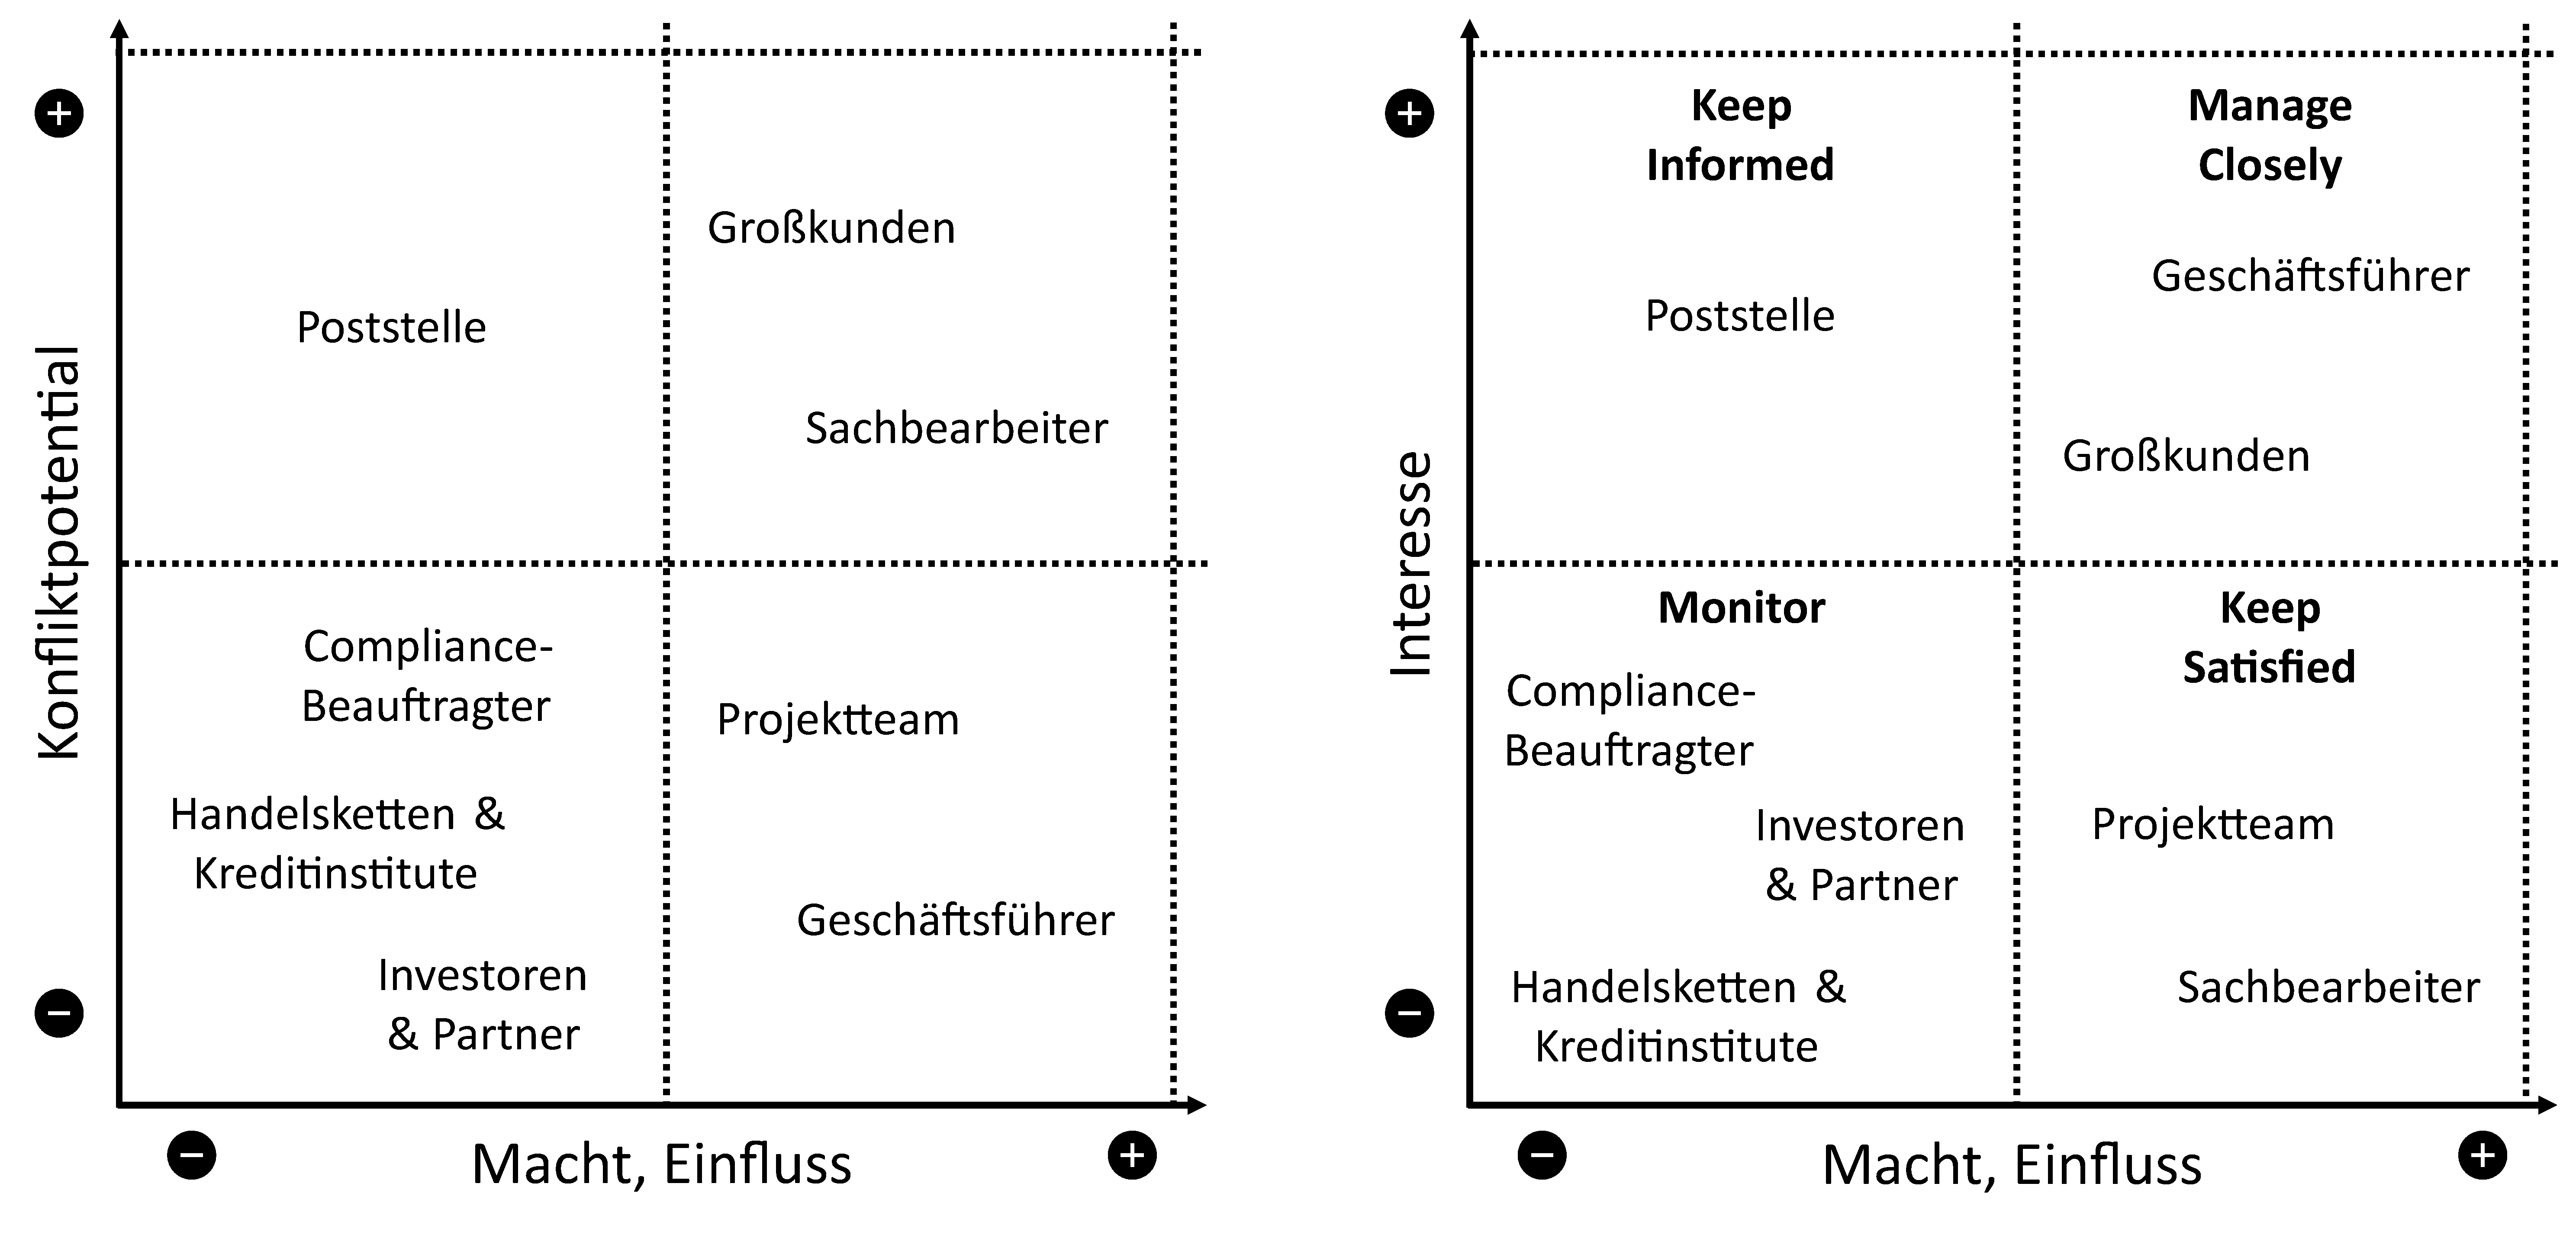
\includegraphics[width=\linewidth]{img/clustering.pdf}
	\caption{Kategorisierung der Stakeholder nach Konfliktpotential, Interesse und Macht}
	\label{fig:macht_cluster}
\end{figure}

Bei der Einteilung zwischen Konfliktpotential und Einflussmöglichkeiten der Stakeholder wird deutlich, dass die Großkunden und Sachbearbeiter über großen Einfluss und ein hohes Konfliktpotential verfügen. Die Großkunden haben die Umsetzung des Projektes vehement gefordert und möchten eigene Anforderungen umgesetzt haben. Durch die bereits erhaltenen Kündigungsdrohungen ist ein hohes Konfliktpotential gegeben. Die Sachbearbeiter hingegen werden nach Fertigstellung des Projekts mit dessen Produkt tagtäglich arbeiten. Somit haben diese einen großen Einfluss auf die Gestaltung, allerdings mit hohem Konfliktpotential, da vermutlich weitergehende, nicht umsetzbare Anforderungen gestellt werden. Die Geschäftsführung und das Projektteam haben ebenfalls einen hohen Einfluss auf das Projekt, allerdings ist das Konfliktpotential überschaubar. Beide Parteien sind direkt an der Projektplanung und dessen Umsetzung beteiligt und können eigene Ideen sofort einbringen. Die Mitarbeiter der internen Poststelle weisen hingegeben ein hohes Konfliktpotential mit relativ geringen Einflussmöglichkeiten auf. Diese sind direkt von den Veränderungen betroffen, da deren Arbeit wegfällt. Allerdings haben sie keine Möglichkeit, etwas hieran zu ändern. Die Investoren \& Partner, Handelsketten \& Kreditinstitute und Compliance-Beauftragte des Unternehmens haben wenig Einfluss und lediglich ein geringes Konfliktpotential, da sie höchstens indirekt durch das Projekt betroffen sind. Folgende Maßnahmen müssen sich daher insbesondere auf die zuvor genannten Stakeholder fokussieren, um deren Konfliktpotential zu minimieren.
\vspace{10pt}

Die Einordnung der Stakeholder bezüglich deren Interesse und Einflussmöglichkeiten ermöglicht eine Zuordnung der Quadranten \textit{Monitor} für wenig Interesse bei geringem Einfluss, \textit{Keep Informed} für viel Interesse bei geringer Macht, \textit{Keep Satisfied} für wenig Interesse bei hoher Macht und \textit{Manage Closely} für viel Interesse bei hoher Macht. Es ergeben sich ähnliche Zusammenhänge im Vergleich zur Kategorisierung nach dem Konfliktpotential, wobei primär die Quadranten \textit{Manage Closely} und \textit{Keep Satisfied} von Relevanz sind. Die Geschäftsführung und Großkunden haben beide direkte Interessen und einen starken Einfluss auf das Projekt. Da die Projektdurchführung von den Großkunden mit Vehemenz gefordert wurde, ist es für die Geschäftsführung von zentraler Bedeutung dieses mit Erfolg umzusetzen. Hingegen befinden sich Projektteam und Sachbearbeiter lediglich im Quadranten \textit{Keep Satisfied}. Für das Projektteam ist dies mit der geringen Dauer des Projekts und der Teamzusammensetzung aus externen und internen Mitarbeitern zu begründen. Die Sacharbeiter haben zudem auch nur ein limitiertes Interesse, da die Umsetzung des Projektes gleichbedeutend mit dem Zwang zur Veränderung und Anpassung ist. Routinen und gelernte Prozesse müssen überarbeitet und neu gelernt werden, weshalb eine gewisse Anfangshürde besteht.
\vspace{10pt}

Basierend auf den identifizierten und analysierten Stakeholdern müssen unterschiedliche Maßnahmen ergriffen werden, um mit diesen in differenzierten Weisen umzugehen. Diese unterscheiden sich in Sofortmaßnahmen und Vorsorgepläne \& Strategien. Hierbei stellen Sofortmaßnahmen Reaktionen auf aktuelle oder unmittelbar bevorstehende Ereignisse oder Probleme dar und müssen daher schnell umgesetzt werden. Sie zielen darauf ab, unmittelbare Risiken zu mindern, Konflikte zu vermeiden und eine positive Beziehung zu den Stakeholdern aufrechtzuerhalten. Vorsorgepläne \& Strategien hingegen beziehen sich auf langfristige Maßnahmen und Pläne, um potenzielle zukünftige Herausforderungen oder Möglichkeiten anzugehen. Die Beziehung zu den Stakeholdern soll über die gesamte Projektlaufzeit positiv und effektiv gestaltet sein. Tabelle \ref{tab:maßnahmen} stellt die Sofortmaßnahmen und Vorsorgepläne \& Strategien als Maßnahmenkatalog dar.
\vspace{10pt}

\begin{longtable}{|p{2.2cm}|p{5.7cm}|p{5.6cm}|}
	\hline 
	\textbf{Stakeholder} & \textbf{Sofortmaßnahmen} & \textbf{Vorsorgepläne \& Strategien} \\
	\hline 
	\endfirsthead
	\multicolumn{3}{c}%
	{\tablename\ \thetable\ -- \textit{Fortsetzung von vorheriger Seite}} \\
	\hline 
	\textbf{Stakeholder} & \textbf{Sofortmaßnahmen} & \textbf{Vorsorgepläne und Strategien} \\
	\hline 
	\endhead
	\hline \multicolumn{3}{r}{\textit{Weiter auf nächster Seite}} \\
	\endfoot
	\hline
	\endlastfoot
	Geschäfts-führung & Einführung in das Projekt und Erläuterung der Ziele und des Zeitplans. & Regelmäßige Updates und Meetings zur Diskussion von Fortschritten und Hindernissen \\
	\hline
	Sach-bearbeiter & Workshops zur Ausarbeitung aller relevanten Anforderungen und Erläuterungen der zu erwartenden Veränderungen & Enge Integration in der Anforderungsaufnahme und im Testen der Anwendung. Schulungen und weitere Unterstützung während des Übergangsprozesses \\
	\hline
	Poststelle & Information über die bevorstehenden Änderungen und Diskussion über die Auswirkungen auf ihre Arbeit & Entwicklung eines Übergangsplans, um die Änderungen zu erleichtern \\
	\hline
	Großkunden & Information über das neue System und dessen Vorteile, Diskussionen und Workshops über deren Bedürfnisse und Erwartungen & Fortlaufende Kommunikation und Unterstützung während des Übergangs, Anpassung des Systems basierend auf deren Feedback \\
	\hline
	Compliance-Beauftragter & Frühzeitige Einbindung in den Planungsprozess, um die Erfüllung aller Datenschutzanforderungen sicherzustellen & Kontinuierliche Überprüfung der Datenschutzmaßnahmen während der Projektumsetzung \\
	\hline
	Projektteam & Bereitstellung von ausreichenden Ressourcen und klare Kommunikation der Projektziele, -erwartungen und -anforderungen & Fortlaufende Unterstützung und Ressourcenmanagement während des gesamten Projekts \\
	\hline
	Externe Partner \& Investoren & Offizielle Mitteilung über das neue Projekt und dessen Ziele & Regelmäßige Updates über den Fortschritt des Projekts \\
	\hline
	Handels-ketten \& Kredit-institute & Offizielle Mitteilung über das neue Projekt und dessen Vorteile & Regelmäßige Updates über den Fortschritt des Projekts \\
	\hline
\end{longtable}
\captionof{table}{Maßnahmenkatalog für Umgang mit Stakeholdern} \label{tab:maßnahmen}
\vspace{20pt}

Für die Kommunikation mit den unterschiedlichen Stakeholdern bedarf es einer Differenzierung in den gewählten Kommunikationsstrategien. Hierbei wird zwischen partizipativem, diskursivem und repressivem Vorgehen unterschieden. Das partizipative Vorgehen bindet den Stakeholder aktiv in Entscheidungsprozesse ein, wodurch das Gefühl der Einflussnahme entsteht. Dies ist von besonderer Relevanz, wenn der Stakeholder direkt von den Entscheidungen betroffen ist oder dessen spezifisches Wissen benötigt wird. Sowohl für die internen Sachbearbeiter, als auch für die Großkunden wird daher das partizipative Vorgehen gewählt, da die Umsetzung derer Anforderungen und die Befriedigung derer Bedürfnisse unerlässlich ist. Für das Projektteam wird ebenfalls dieses Vorgehen gewählt, da es unmittelbar an der Entwicklung und Umsetzung des Projekts beteiligt ist und eine aktive Beteiligung somit gegeben ist. Bei dem diskursivem Vorgehen steht der Austausch und die Diskussionen von Ideen im Vordergrund. Es wird gewählt, wenn die Stakeholder eine hohe Autorität oder Einfluss auf das Projekt haben und unterschiedliche Meinungen hin zu einem Konsens berücksichtigt werden müssen. Diese Kommunikationsstrategie wird daher für die Geschäftsführung genutzt, da diese strategische Entscheidungen trifft, welche umzusetzen sind. Auch für die interne Poststelle und die Datenschutzbeauftragten wird diese Strategie gewählt, um deren Bedenken, Vorschläge und Tipps einbringen zu können. Für die Partner \& Investoren und die Handelsketten \& Kreditinstitute ist diese Strategie ebenfalls von Vorteil, da diese ein Interesse am Projekt haben und sich deren Unterstützung als hilfreich entpuppen kann. Das repressive Vorgehen hingegen nutzt eine intransparente und einseitige Kommunikationsstruktur, um die Offenlegung der Informationen zu verhindern. Da es sich bei unserem Projekt weder um geheime Forschung, noch um anderweitig vertrauliche Themen handelt, wird diese Strategie für keinen Stakeholder verwendet.


\section{Agenda des Kickoff-Workshops}

Basierend auf der durchgeführten Stakeholderanalyse beginnt nun die Planung des Kickoff-Workshops. Alle Schlüsselstakeholder werden zu dem Kickoff-Workshop eingeladen, um Projektziele und Erwartungen zu verdeutlichen und die Zusammenarbeit zu fördern. Dies umfasst die Geschäftsführung, Sachbearbeiter, Großkunden, Datenschutzbeauftragte und das Projektteam. Die Aufgabe der Geschäftsführung während des Kickoff-Workshops liegt in der Erklärung der strategischen Auslegung und Relevanz des Projektes, um alle Teilnehmenden zu motivieren und Unterstützung zu signalisieren. Die Sacharbeiter und Großkunden sind als Endnutzer ebenfalls von Bedeutung, da diese letztendlich mit der entwickelten Lösung arbeiten werden. Bedürfnisse, Anforderungen und Feedback dieser Stakeholder ist daher während des Workshops zu erheben und in der Planung einzuarbeiten. Die Teilnahme des Projektteams ist ebenfalls unverzichtbar, da diese das Projekt umsetzen werden. Während des Workshops können daher Unklarheiten geklärt und Begeisterung für das Projekt geschaffen werden. Auch ein Datenschutzbeauftragter des Unternehmens wird als Unterstützung im Kickoff teilnehmen. Dieser kann sicherstellen, dass alle Datenschutzanforderungen von Beginn an berücksichtigt werden und als Experte für Fragen in diesem Bereich fungieren. Es wird sich bewusst gegen die Einladung von Mitarbeitern der internen Poststelle entschieden, da Arbeitserfahrungen dieser nicht relevant für das Projekt sind. Zudem wären Beitrage der Poststelle eher negativer Natur, da diese um den Verlust ihrer Arbeitsplätze fürchten. Dies würde einen kontraproduktiven Beitrag zum Kickoff-Workshop darstellen, sodass die Produktivität und Effizienz aller Teilnehmenden hierunter leiden würde. Auch externe Partner \& Investoren und Handelsketten \& Kreditinstitute werden aufgrund ihrer Distanz zum Projekt nicht eingeladen. Insgesamt wird mit der Teilnahme von 15 Personen gerechnet, welche sich aus einem Vertreter der Geschäftsführung, dem Projektleiter, drei Vertretern der Großkunden, drei Sachbearbeitern, einem Datenschutzbeauftragten und dem Projektteam der Größe von 6 Mitarbeitern zusammensetzt.
\vspace{10pt}

Bevor die Einladung des Kickoff-Workshop versendet werden kann, muss eine Agenda ausgearbeitet sein. Aufgrund der weiten Anreise mancher Stakeholder wird der Workshop für zwei Tage geplant. Dies ist sinnvoll, da der Kickoff-Workshop wegweisend für das gesamte Projekt ist und eine produktive Zusammenarbeit aller Beteiligten dadurch ermöglicht wird. Der Workshop findet im internen Schulungszentrum der CP Service GmbH statt, welches zahlreiche Ressourcen im Vorhinein bereitstellt. Tabelle \ref{tab:agenda} zeigt die Agenda für den Workshop. Der gesamte Kickoff-Workshop wird durch den Projektleiter Franz Bauer geleitet, um dessen Führungsqualitäten allen Teilnehmern demonstrieren zu können.

\clearpage
\begin{center}
	\Large{\textbf{Tag 1}}
\end{center}

\noindent
\begin{tabularx}{\textwidth}{@{}lX@{}}
	08:30-09:00 & \textbf{Eintreffen der Teilnehmer}\\
	09:00-09:30 & \textbf{Begrüßung und Vorstellung}\\
	& Überblick über den Workshop und die Vorstellung der Teilnehmer.\\
	09:30-10:15 & \textbf{Projektüberblick}\\
	& Präsentation des Projekts, dessen Ziele und des erwarteten Nutzens.\\
	10:15-10:30 & \textbf{Kaffeepause}\\
	10:30-12:00 & \textbf{Diskussion: Projektziele und Erwartungen der Stakeholder}\\
	& Erwartungen und Bedürfnisse der verschiedenen Stakeholder.\\
	12:00-13:00 & \textbf{Mittagspause}\\
	13:00-14:30 & \textbf{Präsentation: Projektplan und -strategie}\\
	& Präsentation des Projektzeitplans und der geplanten Maßnahmen.\\
	14:30-15:00 & \textbf{Kaffeepause}\\
	15:00-16:00 & \textbf{Workshop: Beteiligung der Stakeholder}\\
	& Ausarbeitung von Möglichkeiten der Zusammenarbeit.\\
	16:00-16:30 & \textbf{Closing}\\
	16:30- o.e. & \textbf{[Optional] Gemeinsames Abendessen}
\end{tabularx}


\begin{center}
	\Large{\textbf{Tag 2}}
\end{center}

\noindent
\begin{tabularx}{\textwidth}{@{}lX@{}}
	09:00-09:15 & \textbf{Begrüßung und Überblick}\\
	09:15-10:30 & \textbf{Workshop: Identifizierung möglicher Hindernisse und Risiken}\\
	& Ausarbeitung von Risiken und Entwicklung von Lösungsstrategien.\\
	10:30-10:45 & \textbf{Kaffeepause}\\
	10:45-12:00 & \textbf{Diskussion: Umgang mit Änderungen und Unsicherheiten}\\
	& Änderungsmanagement und der Umgang mit Unsicherheiten.\\
	12:00-13:00 & \textbf{Mittagspause}\\
	13:00-14:30 & \textbf{Diskussion: Verantwortlichkeiten und Rollen im Projekt}\\
	& Rollen und Verantwortlichkeiten der verschiedenen Stakeholder.\\
	14:30-14:45 & \textbf{Kaffeepause}\\
	14:45-16:00 & \textbf{Abschlussdiskussion und nächste Schritte}\\
	& Diskussion der nächsten Schritte und Abschluss des Workshops.\\
\end{tabularx}

\captionof{table}{Agenda für den zweitägigen Kickoff-Workshop}
\label{tab:agenda}
\clearpage

Obwohl der offizielle Beginn des Kickoff-Workshops um 9:00 Uhr ist, muss bereits für die Zeit davor geplant werden. Die Teilnehmer haben eine lange Anreise und werden teilweise bereits vor dem offiziellen Beginn ankommen und einander kennenlernen. Hierfür ist eine entspannte und gemütliche Atmosphäre von Vorteil, sodass die Teilnehmer mit einem positiven Gefühl in den Workshop starten. Es ist wichtig, dass insbesondere für die externen Teilnehmer eine klare Wegbeschreibung zum Schulungszentrum der CP Service GmbH gegeben ist. Diese sollten anschließend von Personal empfangen und zum Raum begleitet werden. Der Projektleiter, welcher den Workshop leiten wird, muss bereits anwesend und der Raum vorbereitet sein. Um eine entspannte Atmosphäre zu schaffen, müssen Snacks, frische Früchte und Getränke jederzeit bereitstehen, um alle Anwesenden zu verpflegen. Der Schulungsraum muss einen großen Tisch in der Mitte haben, an welchen sich alle Teilnehmenden setzen werden. Während beider Tage sind zahlreiche Pausen eingeplant. Diese dienen zum einen der Erholung und Verarbeitung erarbeiteter Themen, sind aber umso wichtiger für das Vernetzen der einzelnen Teilnehmer. Das gesamte Projekt profitiert von einer möglichst guten Zusammenarbeit zwischen den einzelnen Stakeholdern und diese wird durch ein gemeinsames Kennenlernen stark gefördert. 
\vspace{10pt}

Sobald alle Teilnehmer um 9:00 Uhr eingetroffen sind, begrüßt der Projektleiter diese und initiiert eine Vorstellungsrunde. Hierbei ist es wichtig, dass neben beruflichen Aspekten ebenfalls etwas auf private Interessen eingegangen wird, um gemeinsame Gesprächsthemen zu finden und soziale Verbindungen zu knüpfen. Dies soll der emotionalen Auflockerung des Workshops dienen und die Atmosphäre positiv beeinflussen. Nach der Vorstellungsrunde beginnt um 9"30 Uhr der Projektleiter gemeinsam mit der Geschäftsführung einen Überblick über das Projekt, dessen Ziele und den erwarteten Nutzen zu geben. Die Geschäftsführung muss hierbei eine aktive Rolle in der Präsentation einnehmen, um die starke Unterstützung der Führungsspitze zu verdeutlichen. Das Ziel liegt sowohl in der Übermittlung zentraler Projektinformationen, als auch in der Schaffung von Motivation und Begeisterung aller Beteiligter. Nach einer anschließenden Kaffeepause wird um 10:30 Uhr eine aktive Diskussion über Projektziele und Erwartungen der Stakeholder initiiert. Hierbei sollen alle Bedürfnisse offengelegt und klar kommuniziert werden. Dieser Schritt ist von hoher Relevanz, da das Projektteam die konkreten Anforderungen der Großkunden und Sachbearbeiter aufnehmen und verstehen können, sodass eine anschließende Annahme der Anwendersicht möglich wird. Da vermutlich nicht alle Erwartungen umsetzbar sind, muss der Projektleiter als Moderator fungieren und die Diskussion geschickt lenken. Zudem muss sichergestellt werden, dass alle Teilnehmenden aktiv mitarbeiten und nicht einzelne Teilnehmer sämtliche Redeanteile besitzen. Nach der Mittagspause folgt dann um 13:00 Uhr die Präsentation des Projektplans und der Projektstrategie. Der Projektzeitplan wird vorgestellt und geplante Maßnahmen durch den Projektleiter erläutert, sodass alle Teilnehmenden tiefe Einblicke in die Planung erhalten und sich eingebunden fühlen. Da diese Präsentation zahlreiche Informationen vermittelt, wird anschließend eine große Kaffeepause gemacht, in welcher sich die Teilnehmenden auf der Dachterrasse entspannen können. Danach wird noch um 15:00 Uhr ein interaktiver Workshop über die Beteiligung der Stakeholder durchgeführt. Hierbei wird der Projektleiter eine Diskussion über die Rollenverteilung der verschiedenen Stakeholder im Projekt moderieren und gemeinsam mit den Teilnehmenden die Möglichkeiten zur Zusammenarbeit ausarbeiten. Nach diesem Workshop findet um 16:00 Uhr noch das Closing durch den Projektleiter ab, welches die Ergebnisse des ersten Tags zusammenfasst und auf zukünftige Themen eingeht. Dieses Closing beendet den offiziellen Teil des ersten Tages, allerdings wird es für alle Teilnehmenden möglich sein, sich auf ein entspanntes gemeinsames Abendessen in der Stadt zu treffen, um den Tag ausklingen zu lassen.
Nach dem Ende des ersten Tages bereitet der Projektleiter die erzielten Ergebnisse nach und analysiert diese, um langfristig hiervon zu profitieren.
\vspace{10pt}

Der zweite Tag des Kickoff-Workshops beginnt erneut um 9:00 Uhr mit einer Begrüßung durch den Projektleiter. Hierbei wird erneut ein Überblick über bevorstehende Aktivitäten des Tages gegeben, sodass alle Teilnehmenden die Struktur und Organisation des Tages verdeutlicht bekommen. Anschließend beginnt um 9:15 Uhr die Ausarbeitung der Identifikation möglicher Hindernisse und Risiken, um sich dessen bewusst zu werden. Dies ist erneut als aktiver Workshop aufgebaut, in welchem die Teilnehmer ins gemeinsame Gespräch kommen. Risiken und Lösungsstrategien werden gemeinsam ausgearbeitet und anschließend dokumentiert. Der Projektleiter nimmt hierbei eine passivere Rolle an, um den Teilnehmenden mehr Spielraum zu ermöglichen, sodass diese auf neue Ideen kommen können. Nach einer kurzen Kaffeepause wird eine zweite Diskussion um 10:45 Uhr durchgeführt, in welcher es um den Umgang mit Änderungen und Unsicherheiten geht. Die Großkunden und Sachbearbeiter werden starke Veränderungen in ihrem Arbeitsalltag erleben, weshalb diese im Fokus stehen. Es ist auszuarbeiten, inwiefern diese unterstützt und geschult werden können, um die neue Produktlösung nahtlos integrieren zu können. Nach der Mittagspause kommt es um 13:00 Uhr zu einer weiteren Präsentation mit einhergehender Diskussion über die Verantwortlichkeiten und Rollen im Projekt. Hierbei müssen die Befugnisse und Verantwortlichkeiten der einzelnen Stakeholder und deren Einfluss geklärt werden. Es ist erneut wichtig, dass die Geschäftsführung ein positives Bild vermittelt und die vollständige Unterstützung des Projektes signalisiert. Nach einer weiteren Kaffeepause beginnt anschließend die Abschlussdiskussion, in welcher folgende Schritte abgeklärt werden. Nach Abschluss der Diskussion wird anschließend noch Sekt serviert, um den Projektstart zu feiern. Da es sich um den Tag der Abreise handelt und gegebenenfalls manche Teilnehmer noch mit dem Auto fahren, muss ebenfalls eine alkoholfreie Alternative angeboten werden. Der Tag endet somit mit einem positiven Gefühl und alle Teilnehmer können sich auf das Projekt freuen.

\section{Benötigte Materialien}
Der Kickoff-Workshop beinhaltet unterschiedliche Elemente wie Präsentationen, Diskussionen und gemeinsame Ausarbeitungen. Daher ergeben sich diverse benötigte Materialien, welche für den Kickoff-Workshop bereitgestellt werden müssen. Es ist zu beachten, dass die Kaffeemaschine bereits fest installiert ist und das Mittagessen in der Kundenkantine stattfindet, weshalb dies nicht mehr beachtet werden muss. Wie bereits im vorangegangenen Teil beschrieben, wird die Teilnahme von 15 Personen erwartet. Tabelle \ref{tab:materialien} listet alle benötigten Materialien auf, welche für die Organisation des Kickoff-Workshops besorgt werden müssen.
\vspace{10pt}

\begin{table}[h]
	\centering
	\begin{tabular}{|l|l|}
		\hline
		\textbf{Materialien}             & \textbf{Anzahl/Beschreibung} \\
		\hline
		Beamer & 1 \\
		\hline
		Leinwand & 1 \\
		\hline
		Flipchart-Ständer & 3 \\
		\hline
		Flipchart-Papier & Mehrere Blätter \\
		\hline
		Marker (verschiedene Farben) & Mehrere Sätze \\
		\hline
		Post-It Notizen (verschiedene Farben) & Mehrere Päckchen \\
		\hline
		Whiteboard & 1 \\
		\hline
		Whiteboard-Marker & Mehrere Sätze \\
		\hline
		Notizblöcke & 1 pro Teilnehmer \\
		\hline
		Kugelschreiber & 2 pro Teilnehmer \\
		\hline
		Namensschilder & 1 pro Teilnehmer \\
		\hline
		Schilder für die Wegweisung im Gebäude & Mehrere \\
		\hline
		Tische & Ausreichend für alle Teilnehmer \\
		\hline
		Stühle & Ausreichend für alle Teilnehmer \\
		\hline
		Getränke (Wasser, Kaffee, Tee, Säfte) & Ausreichend für alle Teilnehmer \\
		\hline
		Snacks und frische Früchte & Ausreichend für alle Teilnehmer \\
		\hline
		(Alkoholfreier) Sekt für Abschlussfeier & Ausreichend für alle Teilnehmer \\
		\hline
	\end{tabular}
	\caption{Benötigte Materialien für den Kickoff-Workshop}
	\label{tab:materialien}
\end{table}

Neben den benötigten Materialien ist es zusätzlich wichtig, dass weitere Mitarbeiter für die Organisation eingespannt werden. Das Personal des Empfangs muss externe Teilnehmer zum Raum begleiten und es ist zusätzlich ein Praktikant oder Werkstudent notwendig, um bei der kontinuierlichen Dokumentation des Kickoff-Workshops zu unterstützen und ein Protokoll zu führen. Da es sich um einen zweitägigen Workshop handelt und die Vertreter der Großkunden einen weiten Anreiseweg haben, müssen für diese Unterkünfte organisiert werden. Die CP Service GmbH verfügt über ein kleines Kundenhotel in der Nähe des Schulungszentrums. Hier müssen Reservierungen für diese getätigt werden. 


\section{Einladungstext}
Nach der erfolgreichen Stakeholderanalyse, der entwickelten Agenda und ausgearbeiteten Materialien können nun Einladungen an die Stakeholder versendet werden. Da interne Mitarbeiter bereits vor dem Kickoff-Workshop einige Informationen über das Projekt erhalten, dient dieser Einladungstext primär externen Stakeholdern. Es wird versucht einen freundlich bestimmten Schreibstil zu nutzen und die Kompetenzen der einzelnen Stakeholder zu betonen. Es ist wichtig, dass dieser Einladungstext einen positiven Eindruck hinterlässt, sodass der Kickoff-Workshop erfolgreich sein kann. 

\begin{figure}[ht]
	\centering
	\begin{minipage}{\textwidth}		
		\noindent Sehr geehrter [Stakeholder],
		
		\vspace*{1.5\baselineskip}
		
		\noindent wie sie womöglich mitbekommen haben, wollen wir die CP Service GmbH das Projekt Digipaper starten, um Schnittstellen zu digitalisieren. Da wir von Ihrer Kompetenz überzeugt und Ihren Ideen begeistert sind, würden wir Sie sehr gerne zu unserem bevorstehenden \textbf{Kickoff-Workshop} einladen. Dieser findet am \textbf{15. und 16. November 2023} an unserem Hauptstandort in Mannheim statt. 
		
		\vspace*{0.5\baselineskip}
		
		\noindent Dieser Workshop bietet eine wertvolle Gelegenheit, uns gemeinsam auf das spannende Projekt vorzubereiten und unsere \textbf{Ziele und Erwartungen} für die bevorstehenden Monate zu klären. Die Agenda für den Workshop finden Sie im Anhang. 
		
		\vspace*{0.5\baselineskip}
		
		\noindent Während des Workshops wird ein großer Wert auf aktive Beteiligung aller Teilnehmer und deren Meinungen gelegt. Gemeinsam möchten wir die Eckpfeiler des Projekts definieren, unsere Strategie festlegen und mögliche Herausforderungen diskutieren. Sie sind herzlich eingeladen, \textbf{Ihre Ideen und Perspektiven} einzubringen.
		
		\vspace*{0.5\baselineskip}
		
		\noindent Während des Workshops stellen wir Getränke und Snacks sowie ein Mittagessen bereit, um sicherzustellen, dass Sie sich während des ganzen Tages wohlfühlen und konzentrieren können. Sofern eine Unterkunft benötigt wird, sind Sie herzlich dazu eingeladen in unserem Kundenhotel zu übernachten.
		
		\vspace*{0.5\baselineskip}
		
		\noindent Bitte lassen Sie uns bis zum \textbf{10. August 2023} wissen, ob Sie teilnehmen können. Falls Sie von außerhalb anreisen, senden wir Ihnen gerne eine Wegbeschreibung zum Schulungszentrum zu.
		
		\vspace*{0.5\baselineskip}
		
		\noindent Wir freuen uns sehr darauf, Sie bei diesem wichtigen Kickoff-Workshop begrüßen zu dürfen und sind zuversichtlich, dass wir gemeinsam ein erfolgreiches und produktives Projekt starten werden.
		
		\vspace*{1.5\baselineskip}
		
		\noindent Mit freundlichen Grüßen
		
		\vspace*{0.5\baselineskip}
		
		\noindent Franz Urlaub
		
		\noindent Projektleiter
		
		\vspace*{2\baselineskip}
		
		\caption{Einladungsschreiben für den Kickoff-Workshop}
		\label{fig:einladung} 
	\end{minipage}
\end{figure}










% !TEX root = master.tex
\begin{flushleft}
	%\vspace*{0.5cm} 
%\textbf{\LARGE Bewertung potenzieller Risiken}
%\vspace*{0.1cm}
\end{flushleft}

\chapter{Risikomanagement}
\label{chapt:Risikomanagement}
%Erstellt zu eurem Projekt eine Risikoanalyse und betrachtet die Kernrisiken (mind.
%3 Stück) im Detail:
%– Klassifizierung nach Eintrittswahrscheinlichkeit und Auswirkung
%– Erstellung einer geeigneten Visualisierung
%– Beschreibung der Auswirkung auf die Projektdimensionen (-> Risikotyp)
%– Entwicklung geeigneter Maßnahmen und Einordnung in die Maßnahmen-Kategorien
%– Begründung von o.g. Elementen
\label{chapter:6}
\section{Bewertung potenzieller Risiken}
%\textbf{\LARGE Bewertung potenzieller Risiken}
%\vspace*{0.1cm}

Im Rahmen des Risikomanagements wurden 23 potenzielle Risiken identifiziert. Wie diese hinsichtlich ihrer Eintrittswahrscheinlichkeiten und Auswirkungen zu bewerten sind, ist in Abbildung \ref{fig:risikomatrix} visualisiert. Die Zahlen innerhalb der Quadrate entsprechen den Identifikationsnummern der verschiedenen Risiken, welche in Tabelle \ref{tab:risikotb} ausformuliert sind. Der Risikowert ergibt sich aus dem Produkt der Eintrittswahrscheinlichkeit (WSK) und Stärke eines Risikos. 

\begin{figure}[h]
	\centering
	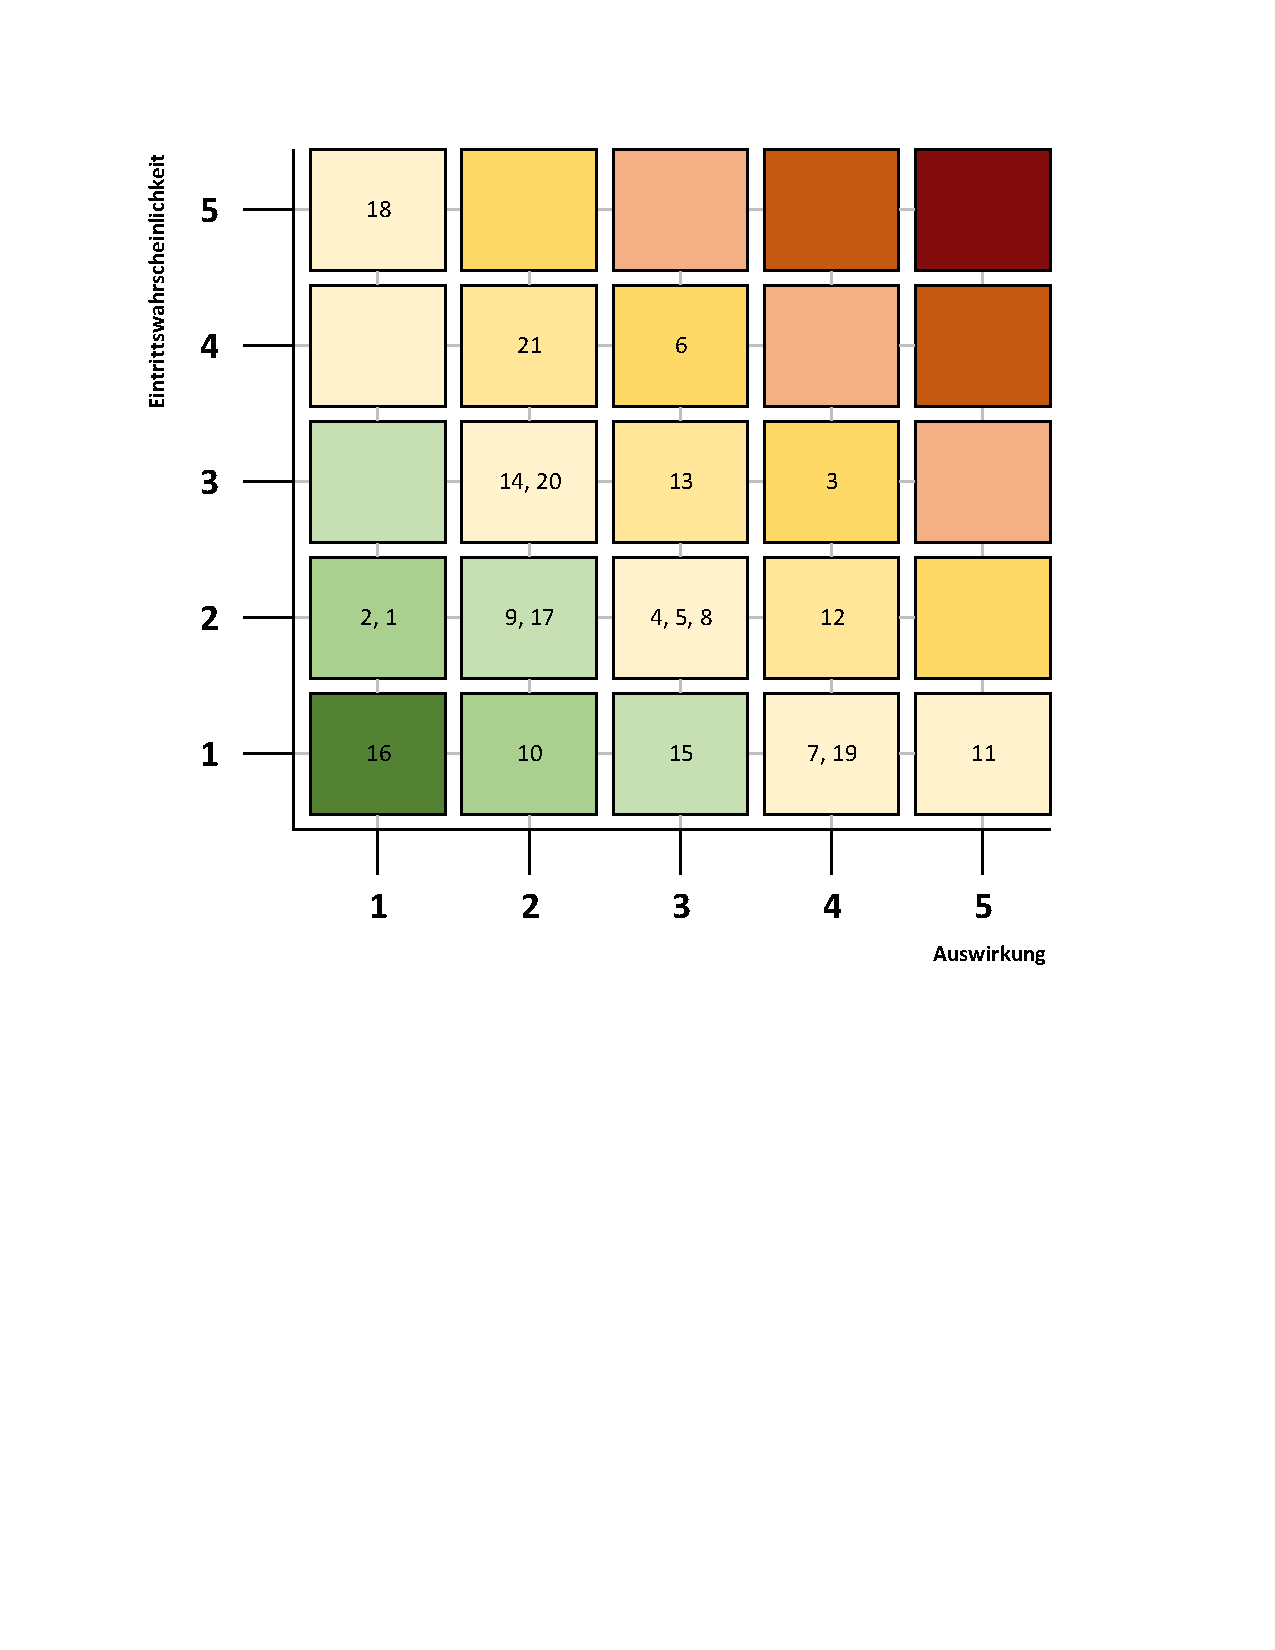
\includegraphics[width=0.85\linewidth]{img/Risikomatrix}
	\caption{Risikomatrix}
	\label{fig:risikomatrix}
\end{figure}


\footnotesize
\newcolumntype{P}[1]{>{\raggedright\arraybackslash}p{#1}}
\newgeometry{left=1cm,right=1cm,top=1cm,bottom=1cm}
\begin{landscape}
	\pagestyle{headings}
	\pagestyle{empty}
	\begin{longtable}{| P{0.5cm} | P{1.7cm} | P{3cm} | P{5cm} | P{1cm} | P{1cm} | P{1cm} | P{2.2cm} | P{2cm} | P{5cm} |}
		
	\hline
	\textbf{ID} &\textbf{Risikotyp}&\textbf{Titel} &\textbf{Beschreibung} &\textbf{WSK} &\textbf{Stärke} &\textbf{Risiko} &\textbf{Problem-Zeitpunkt} &\textbf{Maßnahmen-Kategorie} &\textbf{Maßnahme}\\
	\hline
	\endfirsthead
		
	\multicolumn{10}{c}%
	{\tablename\ \thetable\ -- \textit{Fortsetzung von vorheriger Seite}} \\
	\hline
	\textbf{ID} &\textbf{Risikotyp}&\textbf{Titel} &\textbf{Beschreibung} &\textbf{WSK} &\textbf{Stärke} &\textbf{Risiko} &\textbf{Problem Zeitpunkt} &\textbf{MKategorie} &\textbf{Maßnahme}\\
	\hline
	\endhead
		
	\multicolumn{10}{r}
	{\textit{Weiter auf nächster Seite}} \\
	\endfoot
	\endlastfoot
	
	1&Zeit&Technologie-verschlossenheit&Diffuse Angst vor Veränderungen führt zu fehlender Akzeptanz der Lösung bei den Nutzern&2&1&2&Nach Projektabschluss&Verringern&
	1. Kommunikations- und Schulungsprogramme, um Mitarbeiter über die Vorteile der Digitalisierung aufzuklären und ihre Ängste zu mildern.\\
	\hline

	2&Zeit&Angst vor Arbeitsplatzverlust&Arbeitsplatzverlust (v.a. nach kürzlichem Downsizing) führt zu Widerstand bei Poststellenmitarbeitern&2&1&2&Kickoff bis nach Projektabschluss&Übernehmen&
	1. Regelmäßige Überprüfung des Stimmungsbildes\\
	\hline
	
	3&Leistung&Vernachlässigung der Mitarbeiter-anforderung&Missachtung der Wünsche und Anforderungen der Sachbearbeiter führt zu fehlender Akzeptanz der Lösung&3&4&12&Nach Projektabschluss&Verringern&
	1. Einbeziehung der Mitarbeiter in Planung\newline
	2. Regelmäßige Feedbackschleifen während der Entwicklungsphase\\ 
	\hline

	4&Leistung&Vernachlässigung Kundenanforderung&Missachtung der Wünsche und Anforderungen von Kunden führt zu fehlender Akzeptanz der Lösung&2&3&6&Nach Projektabschluss&Verringern&
	1. Einbeziehung der Kunden in Planung\newline
	2. Regelmäßige Feedbackschleifen während der Entwicklungsphase\\ 
	\hline

	5&Zeit&Fachkräftemangel&Mangelnde Fachkräfte für die Entwicklung bei CP Service GmbH führt zu Ressourcenüberschreitung&2&3&6&Kickoff bis Projektabschluss&Verringern&
	1. Einstellung neuer Mitarbeiter\newline
	2. Weiterbildung bestehender Mitarbeiter\newline
	3. Einbindung externer Berater\\ 
	\hline
	
	6&Zeit&Softwarefehler in Pilotierung&Pilotierung mit fehlerhaftem Produkt führt zu zusätzlichem Entwicklungsaufwand und Missgunst bei Großkunden&4&3&12&Pilotierung&Verringern&
	1. Durchführung gründlicher Tests vor der Pilotierung\newline
	2. Implementierung robuster Unit-, Integrations- und End-to-End-Tests\\
	\hline
	
	7&Kosten&Datenleak&Mangelnder Informationssicherheit führt zu Datenleaks und Strafzahlungen während Pilotierung&1&4&4&Pilotierung&Verringern&
	1. Datenschutzbeauftragten einbinden\newline
	2. Informationssicherheitskonzept erstellen\\ 
	\hline
	
	8&Zeit&Unterschätzung Entwicklungs-aufwand&Unterschätzung des Entwicklungsaufwandes führt zu Ressourcenüberschreitung&2&3&6&Entwicklung bis Pilotierung&Verringern&
	1. Planning Poker mit möglichst allen Projektmitgliedern\newline
	2. Hinreichende Puffer einplanen\\ 
	\hline
		
	9&Leistung&Unklarheit Rollenverteilung&Unklarer Rollendefinitionen führen zu Verantwortungsdiffusion und mangelnder Produktqualität&2&2&4&Entwicklung bis Pilotierung&Verringern&
	1. Klare Rollendefinition mit Kompetenzen\newline
	2. Verantwortung und Aufgaben\\ 
	\hline
	
	10&Zeit&Trotzreaktion&Top-Down-Managementstil und Einmischung in den operativen Betrieb durch die Geschäftsführung führt zu fehlender Akzeptanz bei Mitarbeitern&1&2&2&Nach Projektabschluss&Übernehmen&
	1. Stimmungslage im Blick behalten\\ 
	\hline
	
	11&Leistung&Strategiewechsel&Interner Strategiewechsel führt zu Verlust des Supports vom Top-Management&1&5&5&Kickoff bis Projektabschluss&Übernehmen&
	1. Regelmäßige Überprüfung des Supports durch Top-Management\\ 
	\hline
	
	12&Zeit&Absage Pilotierung&Angst fehlerhaftem Produkt führt dazu, dass die Großkunden nicht an der Pilotierung teilnehmen möchten&2&4&8&Pilotierung&Verringern&
	1. Verhandlung der verbindlichen Teilnahme im Voraus\newline
	2. Übernahme der durch Fehler entstehenden Schäden\\ 
	\hline
		
	13&Zeit&Disharmonie im Team&Fehlende Harmonie (Streit) im Team führt zu längerer Projektlaufzeit&3&3&9&Kickoff bis Projektabschluss&Verringern&
	1. Regelmäßige Retrospektiven\newline
	2. Teambuilding-Maßnahmen\newline
	3. Team-Konstellation konstant halten und Vermittlung während der Storming-Phase\newline
	4. Personenspezifische Maßnahmen zwecks Minimierung des Konfliktpotenzials\\ 
	\hline
	
	14&Zeit&Technische Schwierigkeiten&Technische Schwierigkeiten bei der Entwicklung führen zu Ressourcenüberschreitung&3&2&6&Entwicklung&Verringern&
	1. Externe Hilfe auf Abruf bereithalten\newline
	2. Angemessene Puffer\\
	\hline
	
	15&Zeit&Gesetzesänderung&Veränderte gesetzliche oder regulatorische Vorgaben führen zu Anpassungsbedarf bei Lösung&1&3&3&Kickoff bis Projektabschluss&Übernehmen&
	1. Gesetzeslage im Blick behalten\\ 
	\hline
	
	16&Leistung&Technologie-ablösung&Technologische Innovation führt dazu, dass Lösung bis zum Projektabschluss bereits veraltet ist&1&1&1&Kickoff bis Projektabschluss&Übernehmen&
	1. Technische Entwicklung im Blick behalten\\
	\hline
	
	17&Leistung&Präferenz Papierschnittstelle&Bevorzugung der herkömmlichen Papierschnittstelle führt zu Ablehnung der Lösung bei C- und B-Kunden&2&2&4&Nach Projektabschluss&Übernehmen& 
	1. Intensive Kommunikation der Vorteile\newline
	2. Parallelbetrieb des digitalen und des papierbasierten Prozesses\newline
	3. Verpflichtung zum neuen Prozess\newline
	4. Inkaufnahme von Kündigungen\\ 
	\hline
	
	18&Zeit&Personalausfall&Unvorhergesehener Vorfall (z.B. Krankheit) führt zu Ausfall von Personal&5&1&5&Kickoff bis Projektabschluss&Verringern&
	1. Einplanung ausreichender Puffer\newline
	2. Rechnung mit realistischen Annahmen\\ 
	\hline

	19&Kosten&Softwarefehler in  Rollout&Mangelhaftes Controlling führt zu Rollout mit fehlerhaftem Produkt und Verlust von Kunden&1&4&4&Rollout&Verringern&
	1. Intensives Controlling\newline
	2. Intensives Testing vor Rollout\\ 
	\hline
	
	20&Zeit&Mangelhafte Dokumentation&Mangelhafte Produktdokumentation führt zu eingeschränkten Wartbarkeit und Weiterentwicklung der Lösung nach Projektabschluss&3&2&6&Nach Projektabschluss&Verringern&
	1. Intensives Controlling der Anfertigung der Produktdokumentation\\ 
	\hline
	
	21&Kosten&Transatlantischer Neid&Ausschluss internationaler Kunden vom Rollout führt zu deren Unzufriedenheit/Kündigung aufgrund ungleicher Behandlung&4&2&8&Kickoff bis nach Projektabschluss&Übernehmen&
	1. Stimmungslage im Blick behalten\\ 
	\hline
	

\end{longtable}
\captionof{table}{Risikotabelle} \label{tab:risikotb}
\end{landscape}
\pagestyle{headings}
\restoregeometry
\normalsize

% ----------------
\section{Detailbetrachtung der Kernrisiken}
%\textbf{\LARGE Detailbetrachtung der Kernrisiken}
%\vspace*{0.1cm}

Aufgrund des hohen Zeitdrucks scheint es vertretbar, im Rahmen des Risikomanagements eine Vorauswahl zu treffen. So werden im folgenden nur jene Risiken analysiert, deren Risikowert größer als 7 ist. Die restlichen Eventualitäten werden aufgrund einer geringen Eintrittswahrscheinlichkeit und/oder Stärke zugunsten eines zügigen Projektfortschritts vernachlässigt. Die drohende Insolvenz durch die Kündigung der Großkunden resultiert somit in einer erzwungenen Risikoaffinität bei der CP Service GmbH.


% ---------------- 1 KernRisiko

\vspace*{0.3cm}
\textbf{Risiko 13 - Disharmonie im Team}
\vspace*{0.1cm}

\begin{wrapfigure}{l}{0.15\textwidth}
	
\includegraphics[width=\linewidth]{img/Risikotyp_Zeit}
\end{wrapfigure}

Die Team-Konstellation birgt ein nicht zu vernachlässigendes Konfliktpotenzial. Zunächst gilt es festzustellen, dass der Product Owner Franz Urlaub recht unerfahren und darüber hinaus unbeliebt bei der Belegschaft ist. Dies könnte dazu führen, dass die Team-Mitglieder ihm weniger Respekt entgegenbringen und seine Anweisungen missachten. Sollte es zudem Streit unter den Projektmitgliedern geben, würde Franz Urlaub aufgrund seines Laissez-Faire-Führungsstils nicht eingreifen, was zu einer Eskalation des Konflikt führen könnte. Auch die beiden Scrum-Master könnten in diesem Fall nur bedingt vermitteln, da sie jeweils nur zu 50\% im Projekt involviert sind. Somit fehlt dem Team eine verlässliche zentrale Anlaufstelle, welche die Stimmung einfangen und Auseinandersetzungen präventiv entgegenwirken kann. Konflikte können prinzipiell jederzeit entstehen, im Kontext dieses Projekts sind jedoch zwei Szenarien besonders wahrscheinlich. Zum einen könnte es Streit zwischen Tom Schulze und Harry Mayer geben, weil Tom Wert auf Wissensmanagement und Erfahrungsaustausch legt, während Harry Mayer lieber isoliert für sich arbeitet. Ein weiterer potenzieller Reibungspunkt sind die Unterschiede im Engagement zwischen Stefan Schmitt und Maria Musterfrau. Stefan möchte zukünftig gerne auf eine Teilzeitposition reduzieren, um mehr Zeit mit seiner Familie verbringen zu können, während Maria hoch-engagiert und sehr ehrgeizig am Projekt partizipiert. Der Unterschied in den Prioritäten der beiden Parteien könnte einen Streit auslösen. Sollte Stefan Schmitt noch während des Projekts auf eine Teilzeitstelle wechseln, würde sich das Konfliktpotenzial außerdem insgesamt erhöhen, da die anderen Projektmitglieder seinen Workload übernehmen müssten, was zu Stress und Überlastung führen könnte. Das Risiko lässt sich zwar nicht gänzlich vermeiden, dessen Eintrittswahrscheinlichkeit kann jedoch über die folgenden Maßnahmen reduziert werden:
\begin{itemize}
	\item Zu Beginn der Entwicklungsphase wird von den Scrum-Mastern ein Team-Building-Event durchgeführt, um den Gruppenzusammenhalt zu stärken und die Storming-Phase nach Tuckman zu beschleunigen
	\item Der Product Owner handelt mit Stefan Schmitts Führungsperson noch vor Projektbeginn aus, dass dieser dem Team bis Projektabschluss in Vollzeit erhalten bleibt.
	\item Der Product Owner stellt sicher, dass nicht aus Gründen der Zeitersparnis auf die Retrospektiven am Ende der Sprints verzichtet wird.
\end{itemize}


% ---------------- 2 KernRisiko

\vspace*{0.3cm}
\textbf{Risiko 3 - Vernachlässigung der Mitarbeiteranforderungen}
\vspace*{0.1cm}

\begin{wrapfigure}{l}{0.15\textwidth}
	
\includegraphics[width=\linewidth]{img/Risikotyp_Leistung}
\end{wrapfigure}

Aufgrund der Tatsachen, dass die Geschäftsführung die Kundenzufriedenheit über das Wohl der Mitarbeiter stellt und das Projekt unter großem Zeitdruck durchgeführt wird, ist es wahrscheinlich, dass die Wünsche der Mitarbeiter bei der Konzipierung der digitalen Schnittstelle nicht ausreichend berücksichtigt werden. Dies wäre fatal, da es schon jetzt regelmäßige Beschwerden von Seiten der Sachbearbeiter gibt. Wenn diese nicht in den Entwicklungsprozess eingebunden werden und das Ergebnis des Projekts eine Software-Lösung ist, die nur die Bedürfnisse der Kunden, nicht aber die der internen Nutzer, adressiert, kann dies zu Frust und Ablehnung in der Belegschaft führen. In Kombination mit dem autoritären Top-Down Managementstil der Geschäftsführung und einer gewissen Grundverstimmtheit aufgrund starker Stellenkürzungen innerhalb der letzten drei Jahre, könnte dies eine betriebsschädigende Abwehrhaltung auf Seiten der Arbeitnehmer hervorrufen. Diese Unzufriedenheit könnte sich in der Nicht-Verwendung des neuen Systems und dem Festhalten an alten Prozessen sowie einer langsamen Auftragsabarbeitung oder einer Arbeitsverweigerung manifestieren. Auch wenn die Lösung inhaltlich und qualitativ den in der Planung festgelegte Anforderungen entspricht, lässt sich argumentieren, dass sich ein Eintreten des Risikos dennoch auf die Projektdimension \textit{Leistung} auswirkt, da die Anforderungen der Mitarbeiter nicht enthalten und somit auch nicht erfüllt wurden. Um die Wahrscheinlichkeit für das Eintreten dieses Risikos zu verringern, werden folgende Maßnahmen ergriffen:
\begin{itemize}
	\item Alle Sachbearbeiter werden dazu eingeladen bei der Erstellung des Anforderungskatalogs im Rahmen der Projektplanung mitzuwirken und am Kickoff-Event teilzunehmen. Die Einladung erfolgt über den Product Owner und die Teilnahme ist freiwillig.
	\item Die Sachbearbeiter werden monatlich vom Product Owner per E-Mail über den Stand der Entwicklung informiert und können sich bei Rückfragen an ihn wenden. Dies erzeugt ein Gefühl der Teilhabe, wodurch die Akzeptanz des Endprodukts erhöht wird.
\end{itemize}


% ---------------- 3 KernRisiko

\vspace*{0.3cm}
\textbf{Risiko 12 - Absage Pilotierung}
\vspace*{0.1cm}

\begin{wrapfigure}{l}{0.15\textwidth}
	
\includegraphics[width=\linewidth]{img/Risikotyp_Zeit}
\end{wrapfigure}

Die Idee hinter der Pilotierung ist es, den Großkunden so früh wie möglich die digitale Schnittstelle zur Verfügung zu stellen. Da beim erstmaligen Einsatz eines neuen Systems das Auftreten von Fehlern relativ wahrscheinlich ist, sind die Großkunden eventuell nicht bereit an der Pilot-Phase teilzunehmen. Stattdessen müsste die Pilotierung in Zusammenarbeit mit anderen Kunden erfolgen und die Großkunden würden erst bei der finalen Auslieferung Zugriff auf die Schnittstelle erhalten. Dies führt unweigerlich dazu, dass das Produkt nicht so gut auf die wichtigsten beiden Kunden maßgeschneidert werden kann und verlängert die Zeit bis diese das Produkt erhalten. Mit jeder verstreichenden Woche steigt jedoch die Gefahr, dass die Großkunden die Geduld verlieren und kündigen, da ihre Anliegen nicht schnell genug adressiert wurden. Als Risikotyp wurde die Projektdimension \textit{Zeit} gewählt, weil das oberste Ziel des Projektes die Abwendung der Insolvenz durch den Erhalt der Großkunden darstellt und die Auslieferung an selbige durch deren Verzicht auf die Pilotierung verzögert wird. Folgende Maßnahmen eignen sich, um die Eintrittswahrscheinlichkeit des Risikos zu minimieren:
\begin{itemize}
	\item Der Product Owner verhandelt mit den Großkunden zu Beginn der Planungsphase die Konditionen, welche erfüllt werden müssen, damit sie bereit sind an der Pilotierung teilzunehmen (z.B. 2-wöchiges Testing auf kundenähnlichem System im Vorlauf zur Pilot-Phase)
	\item Optional: Sollten die Sponsoren zustimmen, kann den Großkunden eine Übernahme der durch Bugs entstandenen Schäden angeboten werden.
\end{itemize}

% ---------------- 4 KernRisiko

\vspace*{0.3cm}
\textbf{Risiko 21 - Transatlantischer Neid}
\vspace*{0.1cm}

\begin{wrapfigure}{l}{0.15\textwidth}
	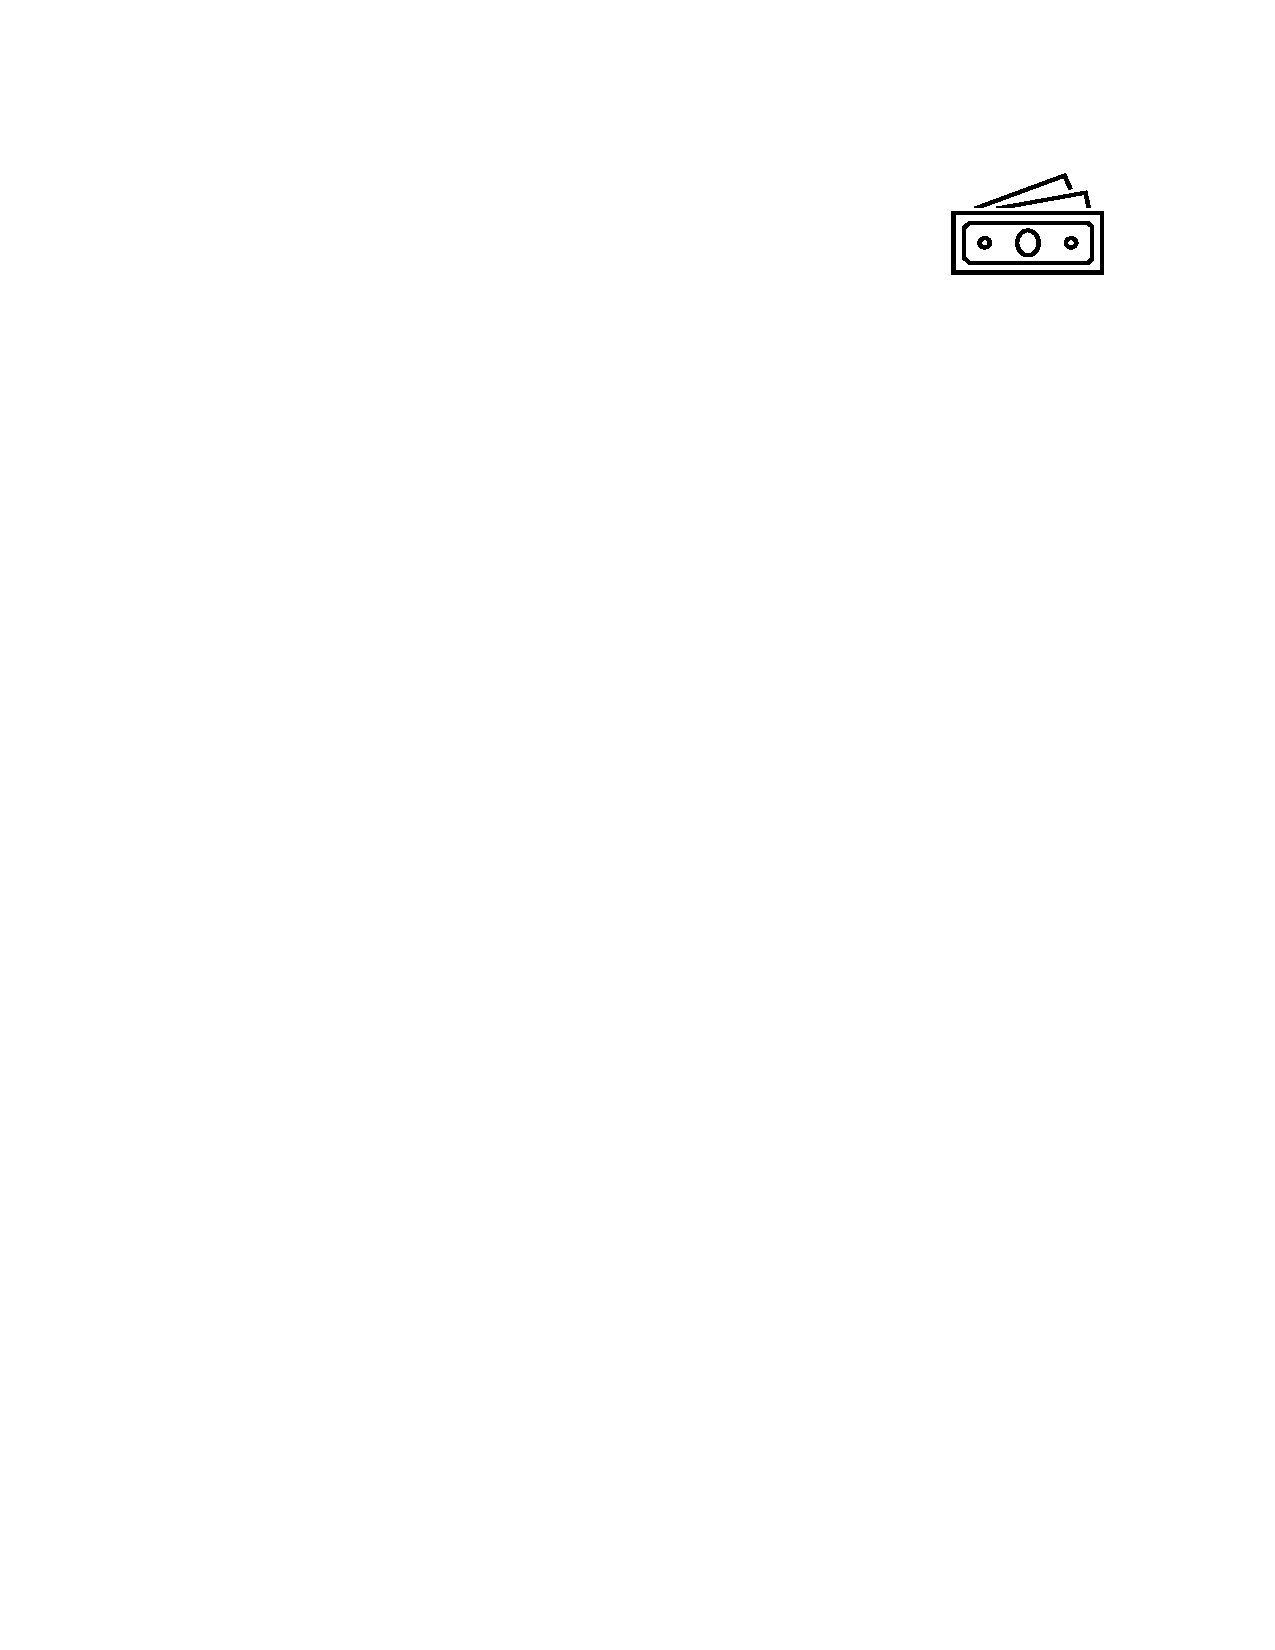
\includegraphics[width=\linewidth]{img/Risikotyp_Kosten}
\end{wrapfigure}

Wie zu Beginn klar definiert wurde, ist der Rollout ausschließlich auf deutsche Kunden begrenzt. Da die Digitalisierung der Schnittstelle jedoch eine signifikante Effizienzsteigerung auf Seiten der Kunden bedeutet und die Verzögerung bei der Abarbeitung von Aufträgen internationale Kunden aufgrund des langen Postweges besonders betrifft, ist es nicht unwahrscheinlich, dass diese zukünftig ebenfalls von der Softwarelösung profitieren wollen. Da es kaum gute Gründe gibt, die internationalen Kunden vom Rollout auszuschließen, wird diese Entscheidung auf Unverständnis stoßen. Dies verschlechtert nicht nur unser Verhältnis zu diesen Kunden, sonder könnte langfristig auch deren Kündigung führen. Dieses Risiko wird von der Projektleitung weder vermieden noch verringert, sondern in Kauf genommen. Folgende Maßnahmen sollten dennoch getroffen werden:

\begin{itemize}
	\item Der Product Owner kommuniziert regelmäßig mit den zuständigen Account Managern, um die Entwicklung der Stimmungslage unserer internationalen Kunden informiert zu sein. 
\end{itemize}


% ---------------- 5 KernRisiko

\vspace*{0.3cm}
\textbf{Risiko 6 - Softwarefehler in Pilotierung}
\vspace*{0.1cm}

\begin{wrapfigure}{l}{0.15\textwidth}
	
\includegraphics[width=\linewidth]{img/Risikotyp_Zeit}
\end{wrapfigure}

Vor dem Hintergrund, dass die Pilot-Phase eines Projekts per Definition der erstmaligen Erprobung risikobehafteter Entwicklungen dient, ist das Auftreten von Softwarefehlern sehr wahrscheinlich. Sollten die Großkunden den Druck auf die Geschäftsführung weiter erhöhen, ist es zudem möglich, dass die Testphase zugunsten einer frühen Auslieferung verkürzt wird, was Wahrscheinlichkeit für das Auftreten von Bugs maßgeblich erhöhen würde. Der Schaden, welcher hierdurch entstehen würde, ist nicht zu unterschätzen. Zum einen wird hierdurch eine Verlängerung des Projekts zur Behebung der Fehler nötig und zum anderen kann es einen erheblichen Imageschaden hervorrufen. Je nach Ausmaß der Anzahl und Größe der Softwarefehler, könnten die Kunden, welche ohnehin bereits unzufrieden mit der von uns erbrachten Leistung sind, sogar eine Kündigung in Betracht ziehen. Zwecks Verringerung der Eintrittswahrscheinlichkeit dieses Risikos werden folgende Maßnahmen ergriffen:
\begin{itemize}
	\item Die geplante Länge der Testphase ist zwingend einzuhalten. Auf Anfrage der Großkunden kommuniziert der Product Owner ihnen detailliert, welche Vorteile sich aus einem ausführlichen Testing für sie ergeben.
	\item Während der Entwicklungsphase werden robuste Unit-, Integration- und End-To-End-Tests implementiert und dokumentiert. Die Tests sind stets von dem Entwickler umzusetzen, welcher für die Realisation der entsprechende Funktionseinheit oder Schnittstelle verantwortlich ist. 
\end{itemize}
% Fazit und Ausblick
%% !TEX root =  master.tex
\chapter{Zusammenfassung}

\nocite{*}

Dieses Kapitel enthält die Zusammenfassung der Arbeit mit Fazit und Ausblick.

\section{Fazit}

...

\section{Ausblick}

...


%%%%%%%%%%%%%%%%%%%%%%%%%%%%%%%%%%%

%%%%%%%%%%%%%%%%%%%%%%%%%%%%%%%%%%%
% ANHÄNGE
%
% @stud: einzelne Anhänge bearbeiten und eigene Anhänge hier einfügen 
%        die nachfolgenden Zeilen deaktivieren, wenn keine Anhänge verwendet werden
%
%\initializeAppendix
%% !TEX root =  master.tex
\chapter{Beispiel-Anhang: Testanhang}

%% !TEX root =  master.tex
\chapter{Beispiel-Anhang: Noch ein Testanhang}
nochmal: lipsum ...

%%%%%%%%%%%%%%%%%%%%%%%%%%%%%%%%%%%

\singlespacing

%%%%%%%%%%%%%%%%%%%%%%%%%%%%%%%%%%%
% LITERATURVERZEICHNIS
% @stud: Literaturverzeichnis in Datei bibliography.bib anpassen. 
%
% Alternative zu Verwendung von \initializeBibliography: Citavi ...
% (dann \initializeBibliography auskommentieren und eigenes LaTex Coding verwenden)
%
\initializeBibliography
%%%%%%%%%%%%%%%%%%%%%%%%%%%%%%%%%%%

%%%%%%%%%%%%%%%%%%%%%%%%%%%%%%%%%%%
% INDEX
% @stud: ggf. Index auskommentieren, wenn nicht benötigt
%
%\addcontentsline{toc}{chapter}{Index}
%\printindex

\end{document}
